\documentclass{article}
\usepackage[utf8]{inputenc}
\usepackage[greek,english]{babel}
\usepackage{alphabeta}
\usepackage{graphicx}
\usepackage{hyperref} 
\usepackage{listings}
\usepackage{subcaption}
\usepackage{mathtools}
\usepackage{tikz}
\usepackage{multirow}
\date{}

















\begin{document}

\begin{titlepage} % Suppresses displaying the page number on the title page and the subsequent page counts as page 1
	
	\raggedleft % Right align the title page
	
	\rule{1pt}{\textheight} % Vertical line
	\hspace{0.05\textwidth} % Whitespace between the vertical line and title page text
	\parbox[b]{0.75\textwidth}{ % Paragraph box for holding the title page text, adjust the width to move the title page left or right on the page
		
		{\Huge\bfseries Τεχνικές \\ \\
		Βελτιστοποίησης\\ \\ }\\[2\baselineskip] % Title
		{\large\textit{ }}\\[4\baselineskip] % Subtitle or further description
		{\Large\textsc{Ιωάννης-Παναγιώτης \\Μπουντουρίδης}} %
	\\	\\{\large\textsc{ΑΕΜ: 8872}} % Author name, lower case for consistent small caps
		
		\vspace{0.5\textheight} % Whitespace between the title block and the publisher
		
		{\noindent \textit{work 1}}\\[\baselineskip] % Publisher and logo
	}

\end{titlepage}
\newpage
\textit{Καθώς οι συναρτήσεις που μας δίνονται είναι κυρτές(σχεδόν κυρτές) και ορισμένες σε ένα διάστημα [a,b]  είναι εμφανές οτι
μπορούμε να χρησιμοποιήσουμε το θεώρημα 5.5.1 και κατ επέκταση, τους αλγορίθμους που
βασίζονται σε αυτό το θεώρημα στη συγκεκριμένη εργασία.}
\section*{Θέμα 1}
\normalsize{}
\subsection*{Λίγα λόγια για τον αλγόριθμο}  
Σε αυτό το θέμα θα υλοποιήσουμε στο matlab τη μέθοδο της διχοτόμου την οποία θα εφαρμόσουμε στις συναρτήσεις και θα σχολιάσουμε τα αποτελέσματα.

Η μέθοδος της διχοτόμου αν και απλή ,οπως θα δούμε είναι μία αργή μέθοδος. Οι παράμετροι που απαιτούνται είναι το $ε$ δηλαδή η απόσταση των $x_1$, $x_2$ από τη διχοτόμο και το $l$ το οποίο δίνει τη συνθήκη τερματισμού δηλαδή, σε τι απόσταση πρέπει να βρίσκονται τα άκρα του διαστήματος ώστε να έχουμε μία ικανοποιητική προσέγγιση του ελαχίστου της συνάρτησης. \\
\subsection*{Περιγραφή αλγόριθμου}
Ο αλγόριθμος της διχοτόμου δεδομένων των $ε>0$ και $l>0$ ξεκινάει με το αρχικό διάστημα $[a_1,b_1]$ και σε ένα βρόγχο (while) με συνθήκη τερματισμού $\boxed{ b_k - a_k < l}$ επιλέγει τα σημεία
\begin{equation*}
\boxed{x_{1k} = \frac{a_k+b_k}{2} - ε} \enspace \boxed{x_{2k} = \frac{a_k+b_k}{2} + ε}
\end{equation*}
Αν $\boxed{f(x_{1k}) < f(x_{2k}) \Rightarrow a_{k+1} = a_k \enspace και \enspace b_{k+1} = x_{2k}}$ \\
διαφορετικά $\boxed{f(x_{1k}) > f(x_{2k}) \Rightarrow a_{k+1} = x_{1k} \enspace και \enspace b_{k+1} = b_k}$\\
\subsection*{Υπολογισμοί της αντικειμενικής συνάρτησης}
Όπως φαίνεται στην περιγραφή του αλγόριθμου σε κάθε επανάληψη υπολογίζουμε τις μεταβλητές $x_{1k}$ και $x_{2k}$ ώστε να προκύψει ανάλογα με την περίπτωση $f(x_{1k}) < f(x_{2k})$ ή $f(x_{1k}) > f(x_{2k})$ το νέο εύρος $[a_k,b_k]$. Για k=1 δεν έχουμε κανένα υπολογισμό της αντικειμενικής συνάρτησης ενω για k=2 έχουμε δύο υπολογισμούς $f(x_1)$ και $f(x_2)$ για τον έλεγχο της συνθήκης. Kαταλήγουμε οτι oι υπολογισμοί της αντικειμενικής συνάρτησης συνδέονται απο την σχέση:
\begin{equation*}
\boxed{calc(k) = 2(k-1)} 
\end{equation*}
\newpage
\subsection*{Σταθερό $l$}
 
Για σταθερό τελικό εύρος αναζήτησης $\boxed{l=0.01}$ μελετάμε τη μεταβολή των υπολογισμών της αντικειμενικής συνάρτησης καθώς μεταβάλλουμε την απόσταση απο τη διχοτόμο (δηλαδή την μεταβλητή ε) 
\par{} Για $\boxed{0.00009\leq ε \leq 0.00049}$ επιλέγουμε 51 σημεία.\\
\begin{figure*}[h!]	
     \centering  
     \advance\leftskip-2.9cm  
  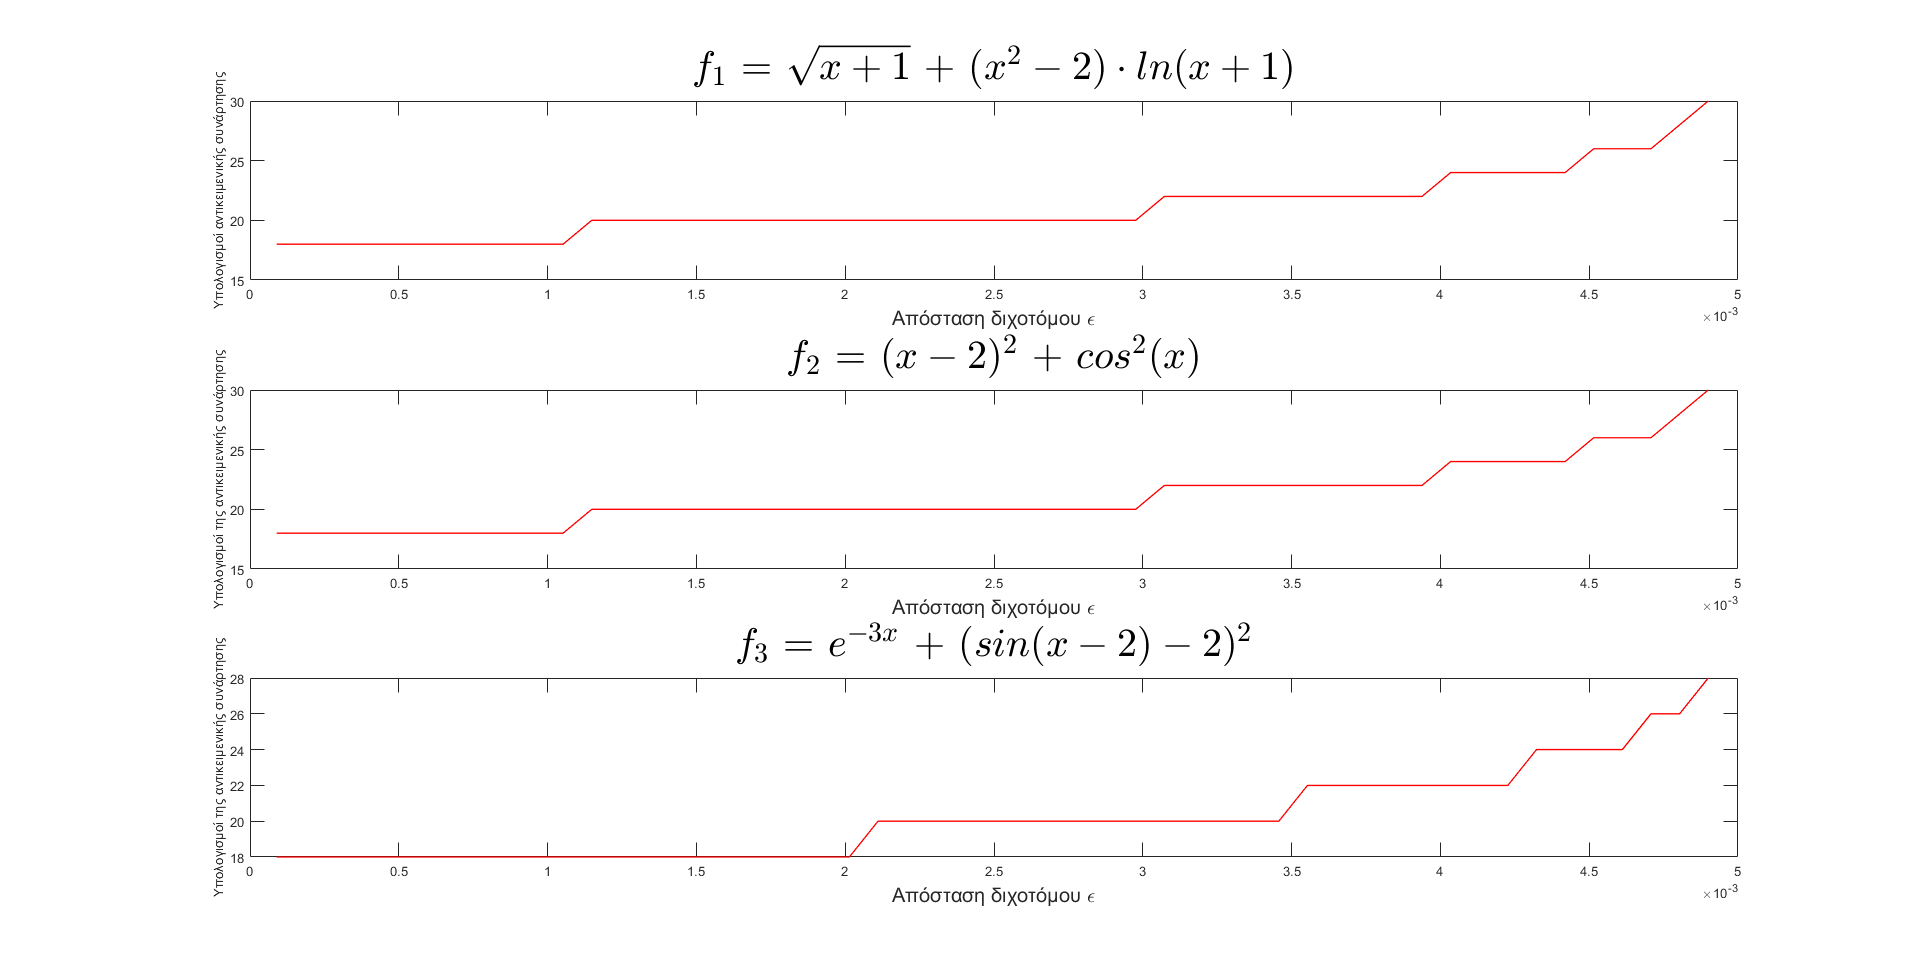
\includegraphics[width=180mm,scale=2]{thema1a.png}
\end{figure*} 


 Παρατηρούμε οτι για $\boxed{ε\geq l/2}$ ο αλγόριθμος δεν τερματίζει ενώ για τιμές κοντά στο $\boxed{ε=l/2}$ η επαναλήψεις αυξάνονται σημαντικά. 
\newpage
\subsection*{Σταθερό $ε$}
Αντίστοιχα για σταθερό $\boxed{ε=0.001}$ οσο μεγαλώνει το $l$ τόσο μειώνονται οι επαναλήψεις.
\begin{figure*}[h!]	
     \centering
     \advance\leftskip-2.9cm  
  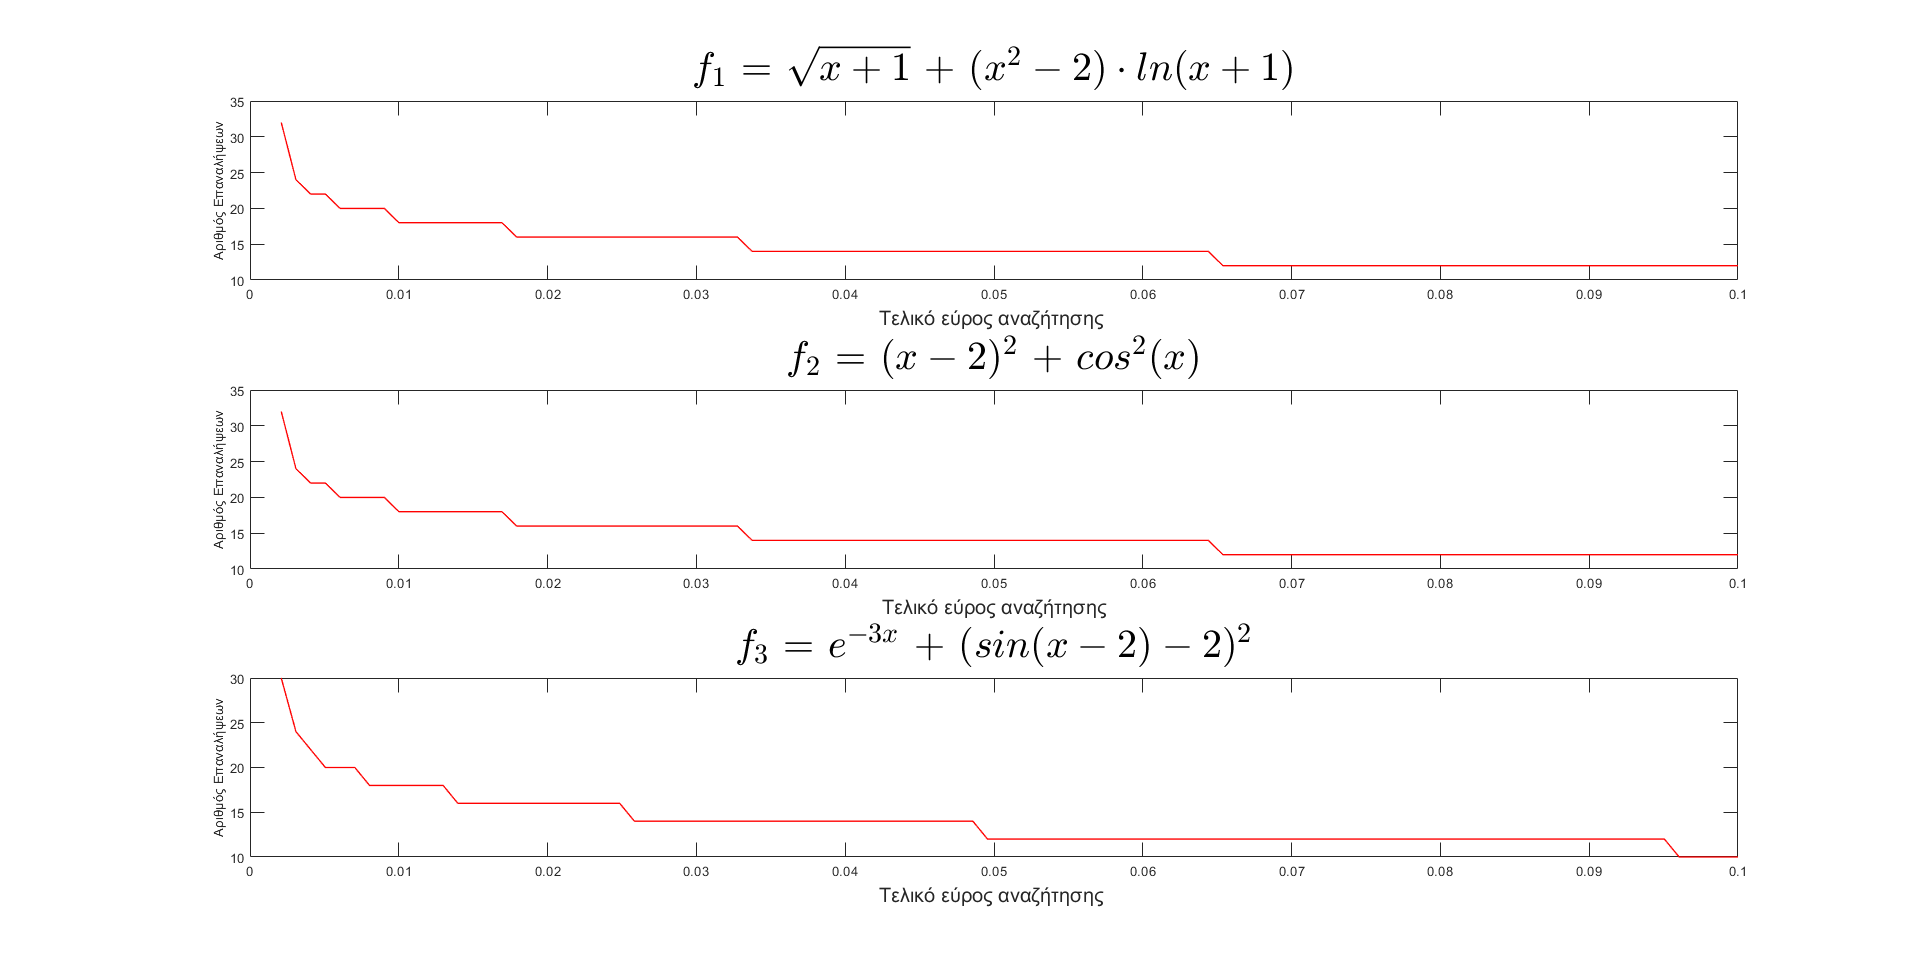
\includegraphics[width=180mm,scale=2]{thema1b.png}
\end{figure*}

O αριθμός των υπολογισμών της αντικειμενικής συνάρτησης ικανοποιεί την σχέση: $\boxed{n \geq 2 \cdot log_2(\frac{b_1-a_1}{l-ε})}$ ενώ οπως αποδείξαμε πιο πάνω ο αριθμός των κλήσεων n συνδέεται με τον αριθμό των επαναλήψεων $k$ με την σχέση: $\boxed{n = 2(k-1)}$
\newpage
\subsection*{Μεταβολή των υποδιαστημάτων $[a_k,b_k]$}
Tέλος παρουσιάζονται τα διαστήματα $[α_k,b_k]$ ανα επανάληψη $k$ για διάφορα $l$  
\begin{figure*}[h!]	
     \centering
     \advance\leftskip-2.45cm 
  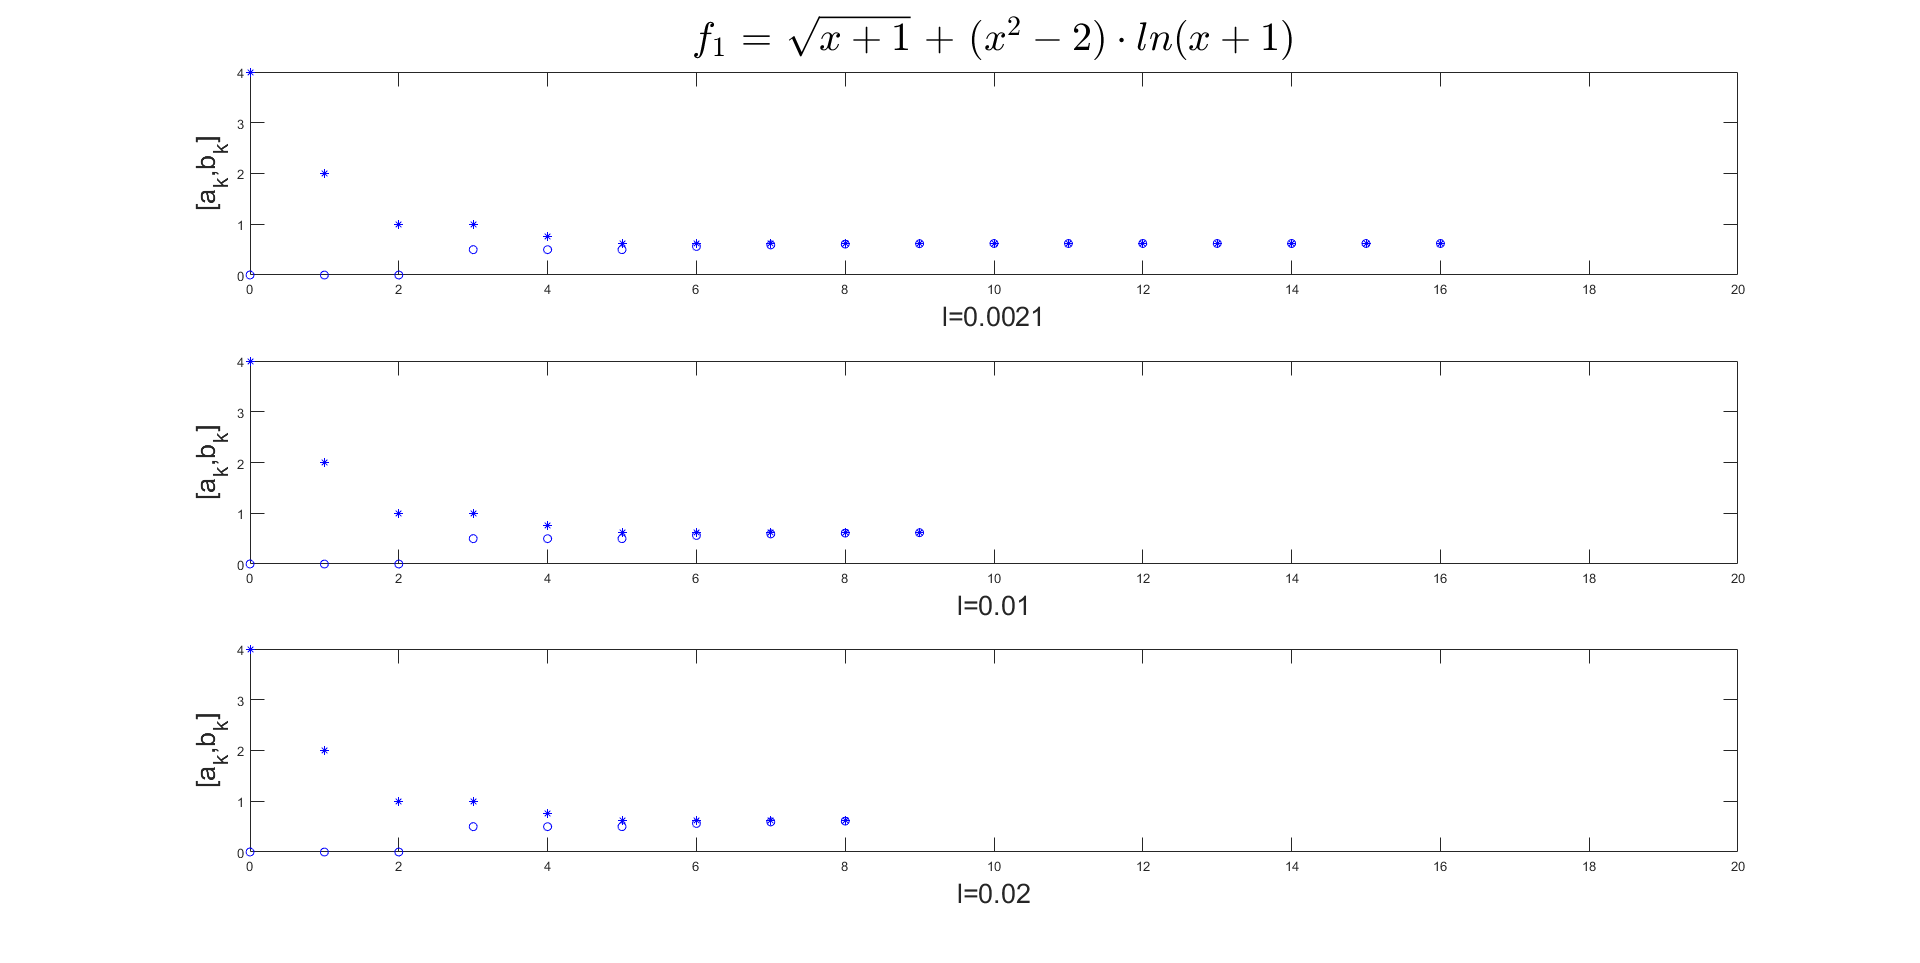
\includegraphics[width=160mm,scale=2]{t3a.png}
\end{figure*}

\begin{figure*}[h!]	
     \centering
     \advance\leftskip-2.45cm 
  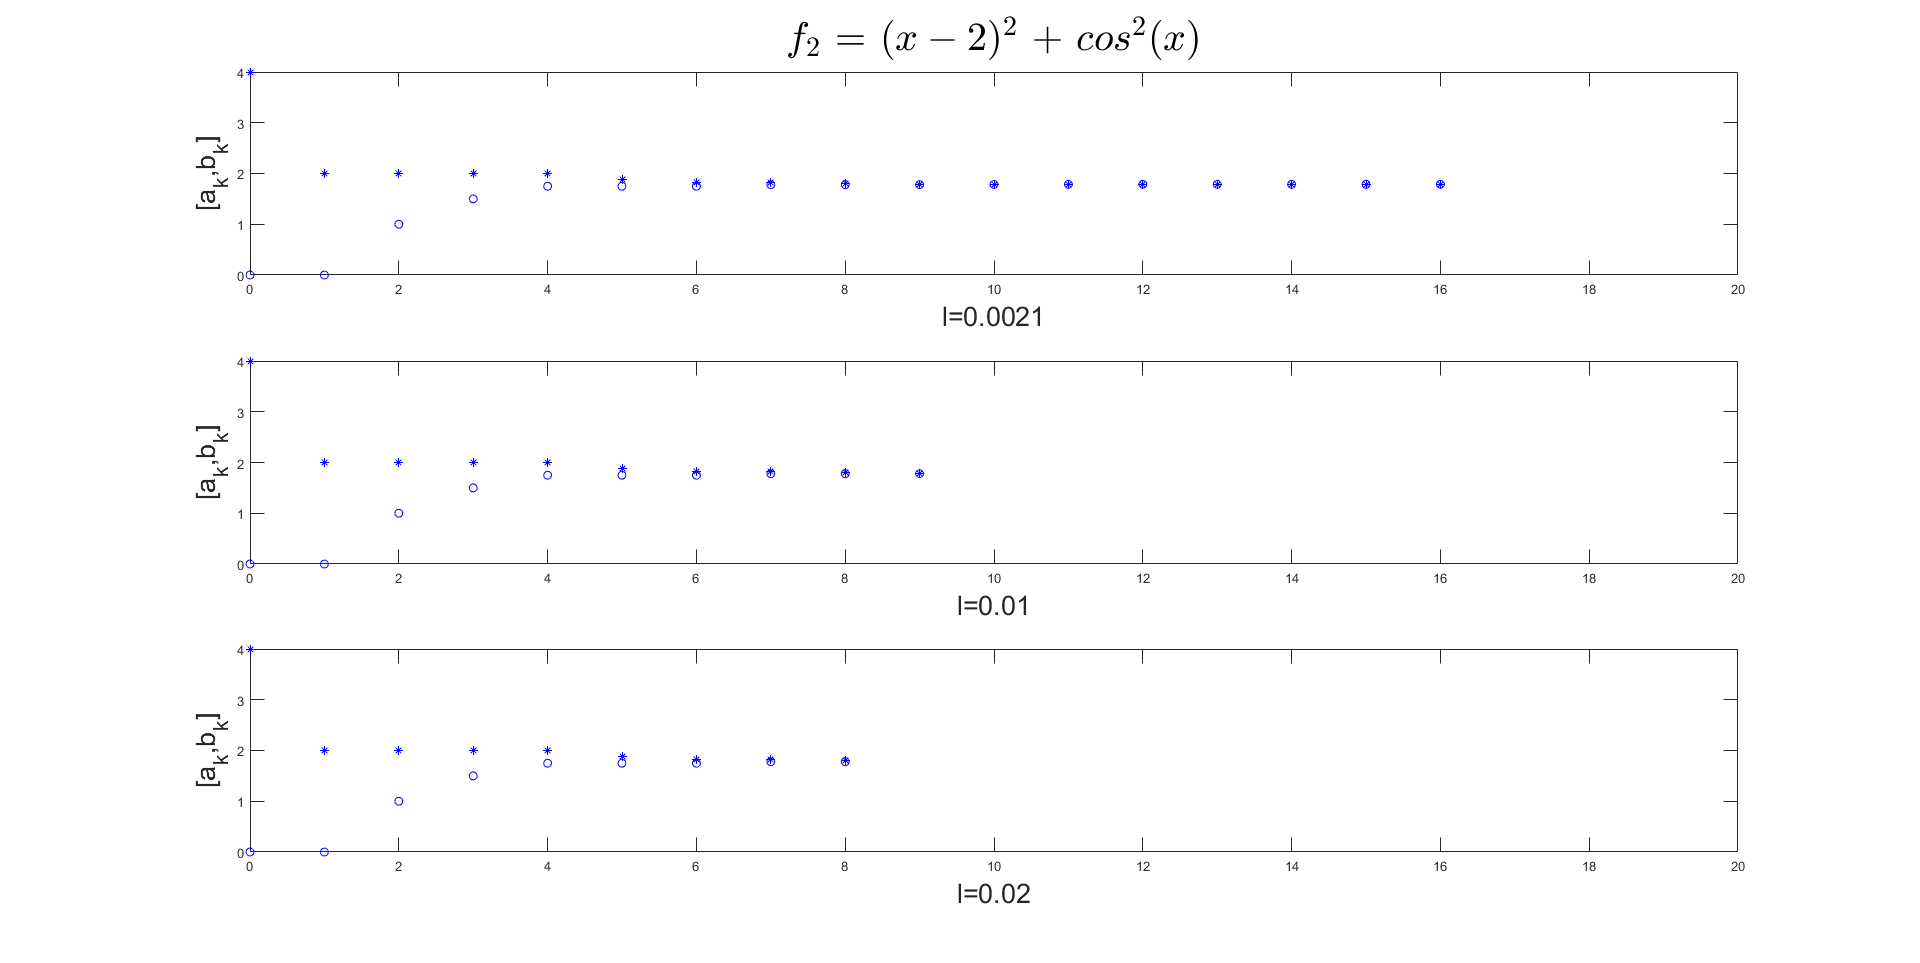
\includegraphics[width=160mm,scale=2]{t3b.png}
\end{figure*}
\clearpage
\begin{figure*}[h!]	
     \centering
     \advance\leftskip-2.45cm 
  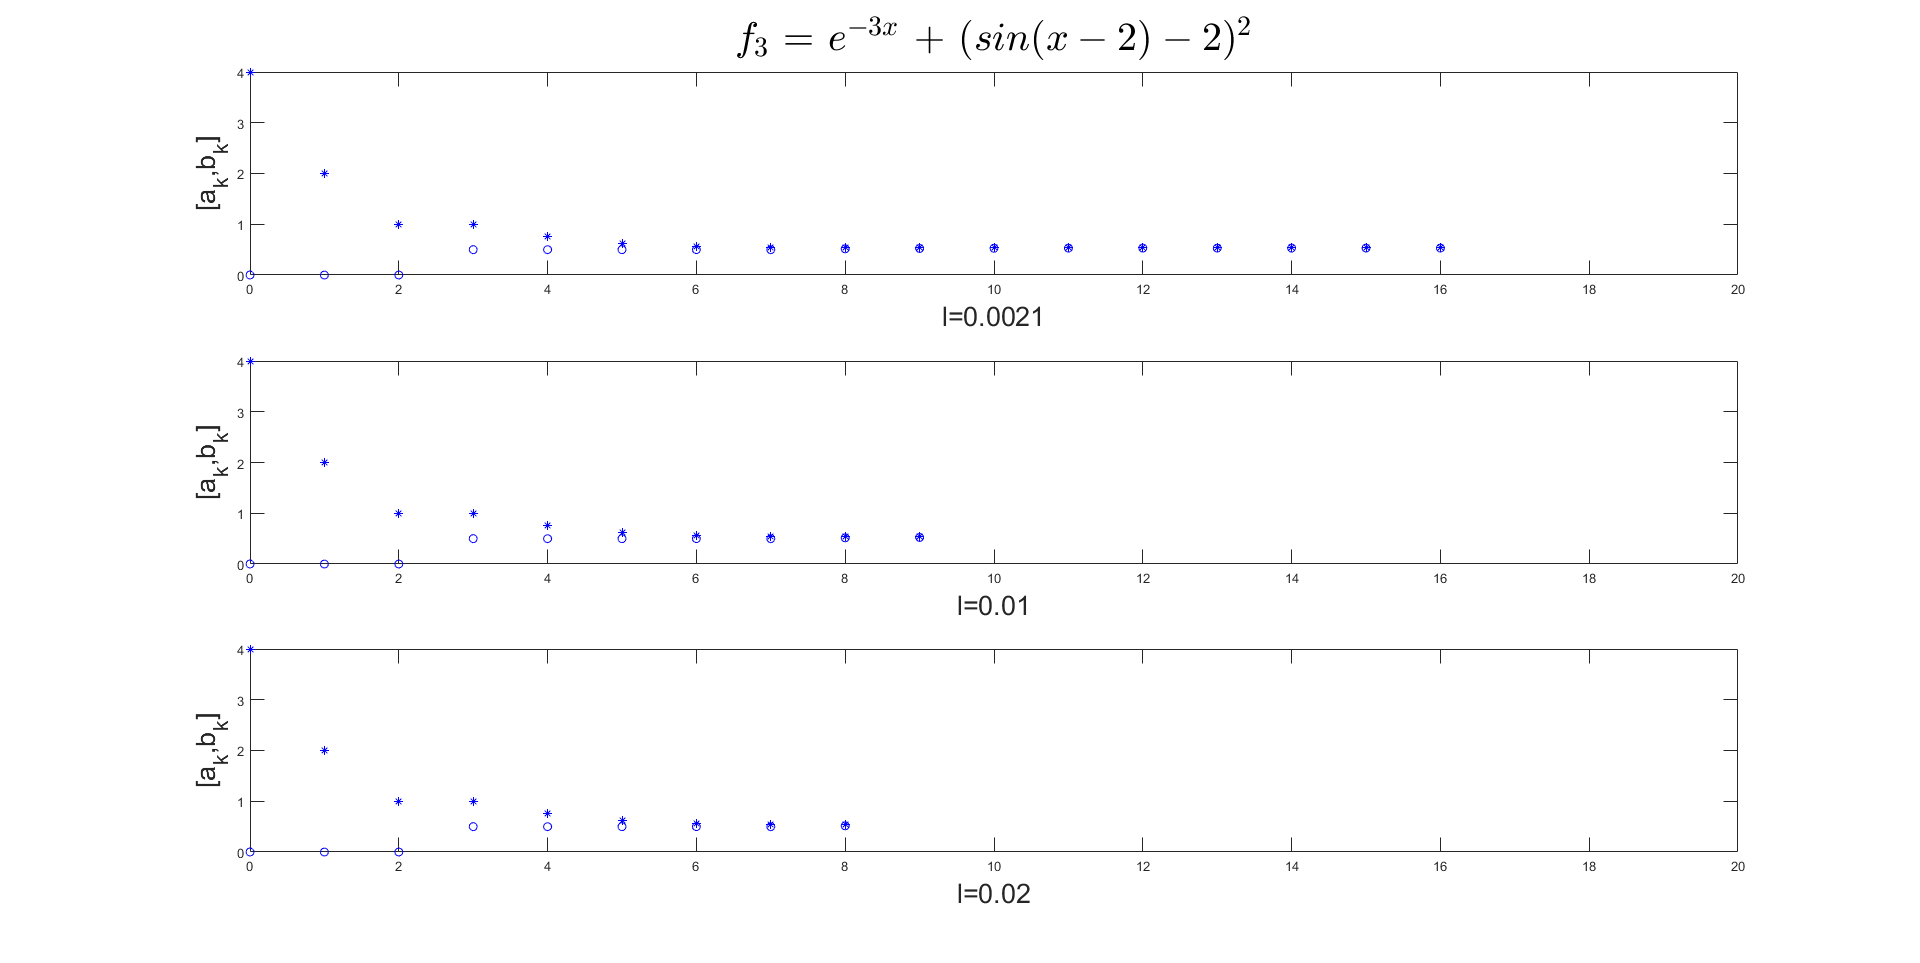
\includegraphics[width=170mm,scale=2]{t3c.png}
\end{figure*}
Όπως φαίνεται απο τα διαγράμματα ο αλγόριθμος συγκλίνει στο ελάχιστο πιο γρήγορα οσο το $l$ μεγαλώνει με μικρότερη ακρίβεια για σταθερό $ε=0.001$ \\ 
Βλέπουμε ότι όσο πιο μικρό l δηλαδή όσο μεγαλύτερη ακρίβεια απαιτείται στην εύρεση του
ελαχίστου, τόσο αυξάνονται και οι επαναλήψεις του αλγόριθμου μέχρι τον τερματισμό του, κάτι
απολύτως λογικό.
\newpage
\section*{Θέμα 2}
\subsection*{Λίγα λόγια για τον αλγόριθμο} 
Σε αυτό το θέμα θα υλοποιήσουμε στο matlab τη μέθοδο του χρυσού τομέα την οποία θα εφαρμόσουμε στις συναρτήσεις και θα σχολιάσουμε τα αποτελέσματα.

Η μέθοδος του χρυσού τομέα βασίζεται και αυτή στη λογική ότι έχουμε ένα αρχικό διάστημα
[a,b] και προσπαθούμε να το περιορίζουμε(συνεχώς μέχρι να τερματιστεί ο αλγόριθμος) και στο
τελικό διάστημα(όπως και σε όλα τα προηγούμενα διαστήματα) να περιέχεται το ελάχιστο της
συνάρτησης με ακρίβεια l(απόσταση των άκρων a, b)  \\
Η βασική ιδιότητα που συνδέει το νέο
υποδιάστημα με το προηγούμενο είναι $b_{k+1}-a_{k+1}=γ(b_k -a_k)$ όπου γ ίσο με 0.618 και $a_k$ , $b_k$ τα άκρα του διαστήματος

\subsection*{Περιγραφή αλγόριθμου}
Ο αλγόριθμος του χρυσού τομέα δεδομένου του τελικού εύρους $l>0$ για αρχικό διάστημα $[a_1,b_1]$ αρχικοποιεί τα σημεία
\begin{equation*}
\boxed{x_{11} =  a_1 + (1-γ)(b_1-a_1) } \enspace \boxed{x_{21} =  a_1 + γ(b_1-a_1)} 
\end{equation*}
με γ = 0.618 σε ένα βρόγχο (while) με συνθήκη τερματισμού $\boxed{ b_k - a_k < l}$ επιλέγει τα σημεία \\
αν $\boxed{f(x_{1k}) > f(x_{2k}) \Rightarrow a_{k+1} = x_{1k} \enspace και \enspace b_{k+1} = b_{k}}$ \\
τα σημεία ανανεώνονται σε: $\boxed{x_{2k+1} = a_{k+1} + γ(b_{k+1} - a_{k+1})\enspace και\enspace x_{1k+1} = x_{2k}}$  \\
αν $\boxed{f(x_{1k}) < f(x_{2k}) \Rightarrow a_{k+1} = a_{k} \enspace και \enspace b_{k+1} = x_{2k}}$ \\
τα σημεία ανανεώνονται σε: $\boxed{x_{1k+1} = a_{k+1} + (1-γ)(b_{k+1} - a_{k+1})\enspace και\enspace x_{2k+1} = x_{1k}}$ 

 
 \subsection*{Υπολογισμοί της αντικειμενικής συνάρτησης}
Οπως είδαμε στην παραπάνω περιγραφή στην αρχή του αλγορίθμου υπολογίζουμε αρχικά τα σημεία $x_{11}$ και $x_{21}$ αρα και κατ επέκταση τα $f( x_{11})$ και $f( x_{21})$ δηλαδή έχουμε δύο υπολογισμούς της αντικειμενικής συνάρτησης για την πρώτη επανάληψη ενώ για τις επόμενες επαναλήψεις προστίθεται μόνο ένας υπολογισμός της αντικειμενικής συνάρτησης ανάλογα με την περίπτωση $f(x_{1k}) < f(x_{2k})$ ή $f(x_{1k}) > f(x_{2k})$ . \\
Kαταλήγουμε οτι oι υπολογισμοί της αντικειμενικής συνάρτησης συνάρτηση του k συνδέονται απο την σχέση:
\begin{equation*}
\boxed{calc(k) = k+1} 
\end{equation*}
Για k=1 έχουμε έχουμε δύο υπολογισμούς της αντικειμενικής συνάρτησης αφού υπολογίζουμε τα $f( x_{11})$ και $f( x_{21})$. Όμοια για k = 2 έχουμε τρείς υπολογισμούς της αντικειμενικής συνάρτησης αφού σε κάθε επόμενη επαναληψη μετά της πρώτης έχουμε εναν επιπλέον υπολογισμό. \newpage
\subsection*{Μεταβολή τελικού ευρους αναζήτησης}
Παρακάτω μελετάμε τη μεταβολή των υπολογισμών της αντικειμενικής συνάρτησης $f_i(x)$
καθώς μεταβάλλουμε το τελικό εύρος αναζήτησης l.
\begin{figure*}[h!]	
     \centering
     \advance\leftskip-4.75cm 
  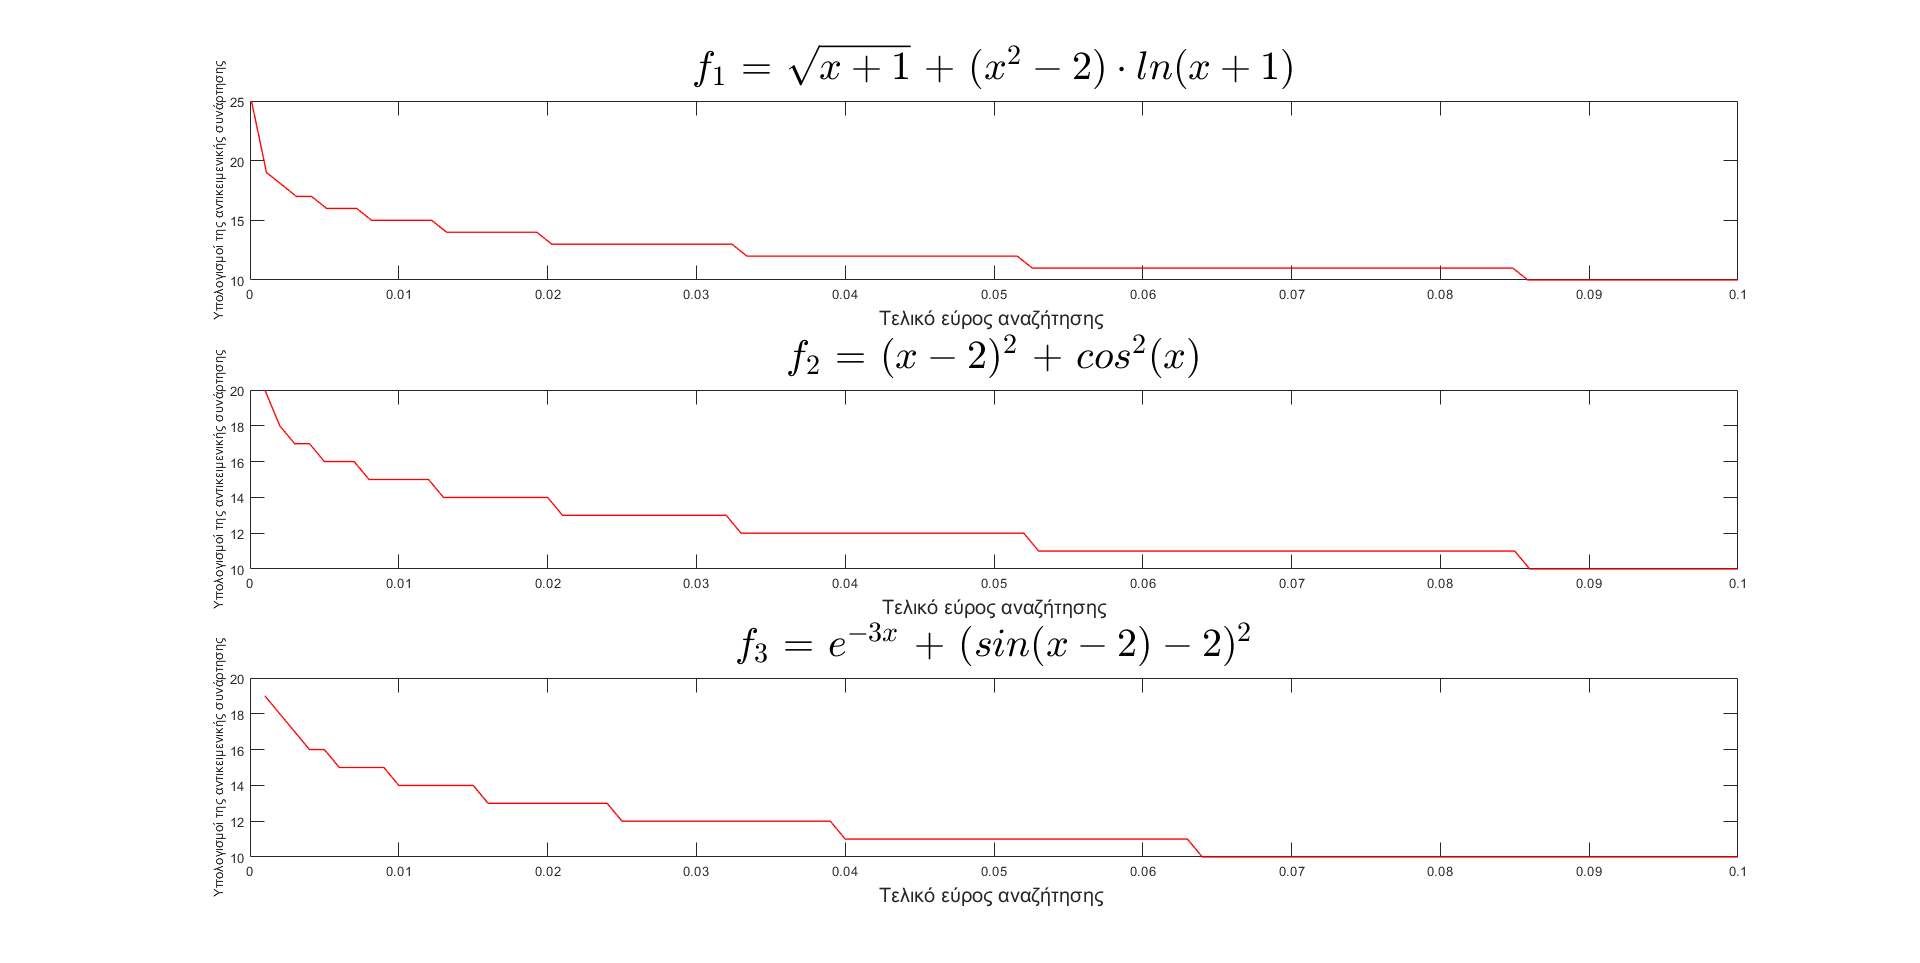
\includegraphics[width=220mm,scale=2]{thema2a.png}
\end{figure*} \\
Βλέπουμε ότι όσο πιο μικρό l δηλαδή όσο μεγαλύτερη ακρίβεια απαιτείται στην εύρεση του
ελαχίστου, τόσο αυξάνονται και οι επαναλήψεις του αλγόριθμου μέχρι τον τερματισμό του, κάτι
απολύτως λογικό.
 \clearpage
 \subsection*{Μεταβολή των υποδιαστημάτων $[a_k,b_k]$}
Tέλος παρουσιάζονται τα διαστήματα $[α_k,b_k]$ ανα επανάληψη $k$ για διάφορα $l$  
\begin{figure*}[h!]	
     \centering
     \advance\leftskip-2.45cm 
  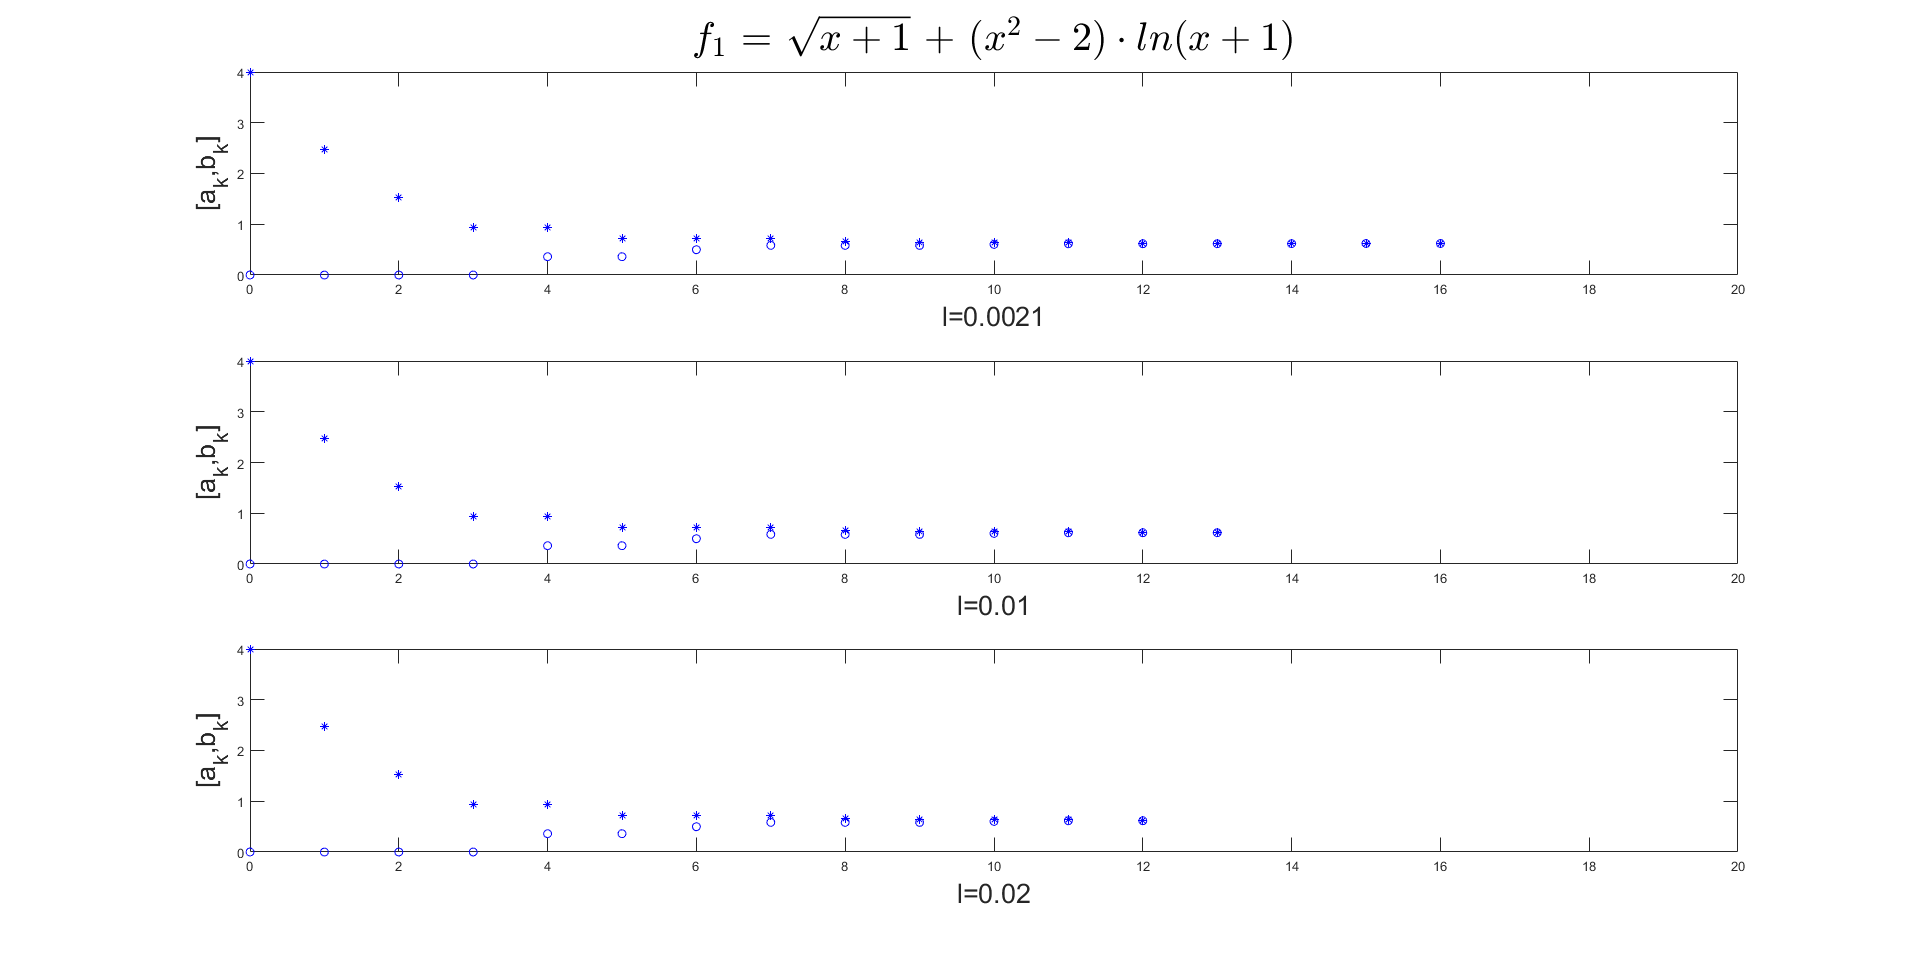
\includegraphics[width=160mm,scale=2]{u2a.png}
\end{figure*}
\begin{figure*}[h!]	
     \centering
     \advance\leftskip-2.45cm 
  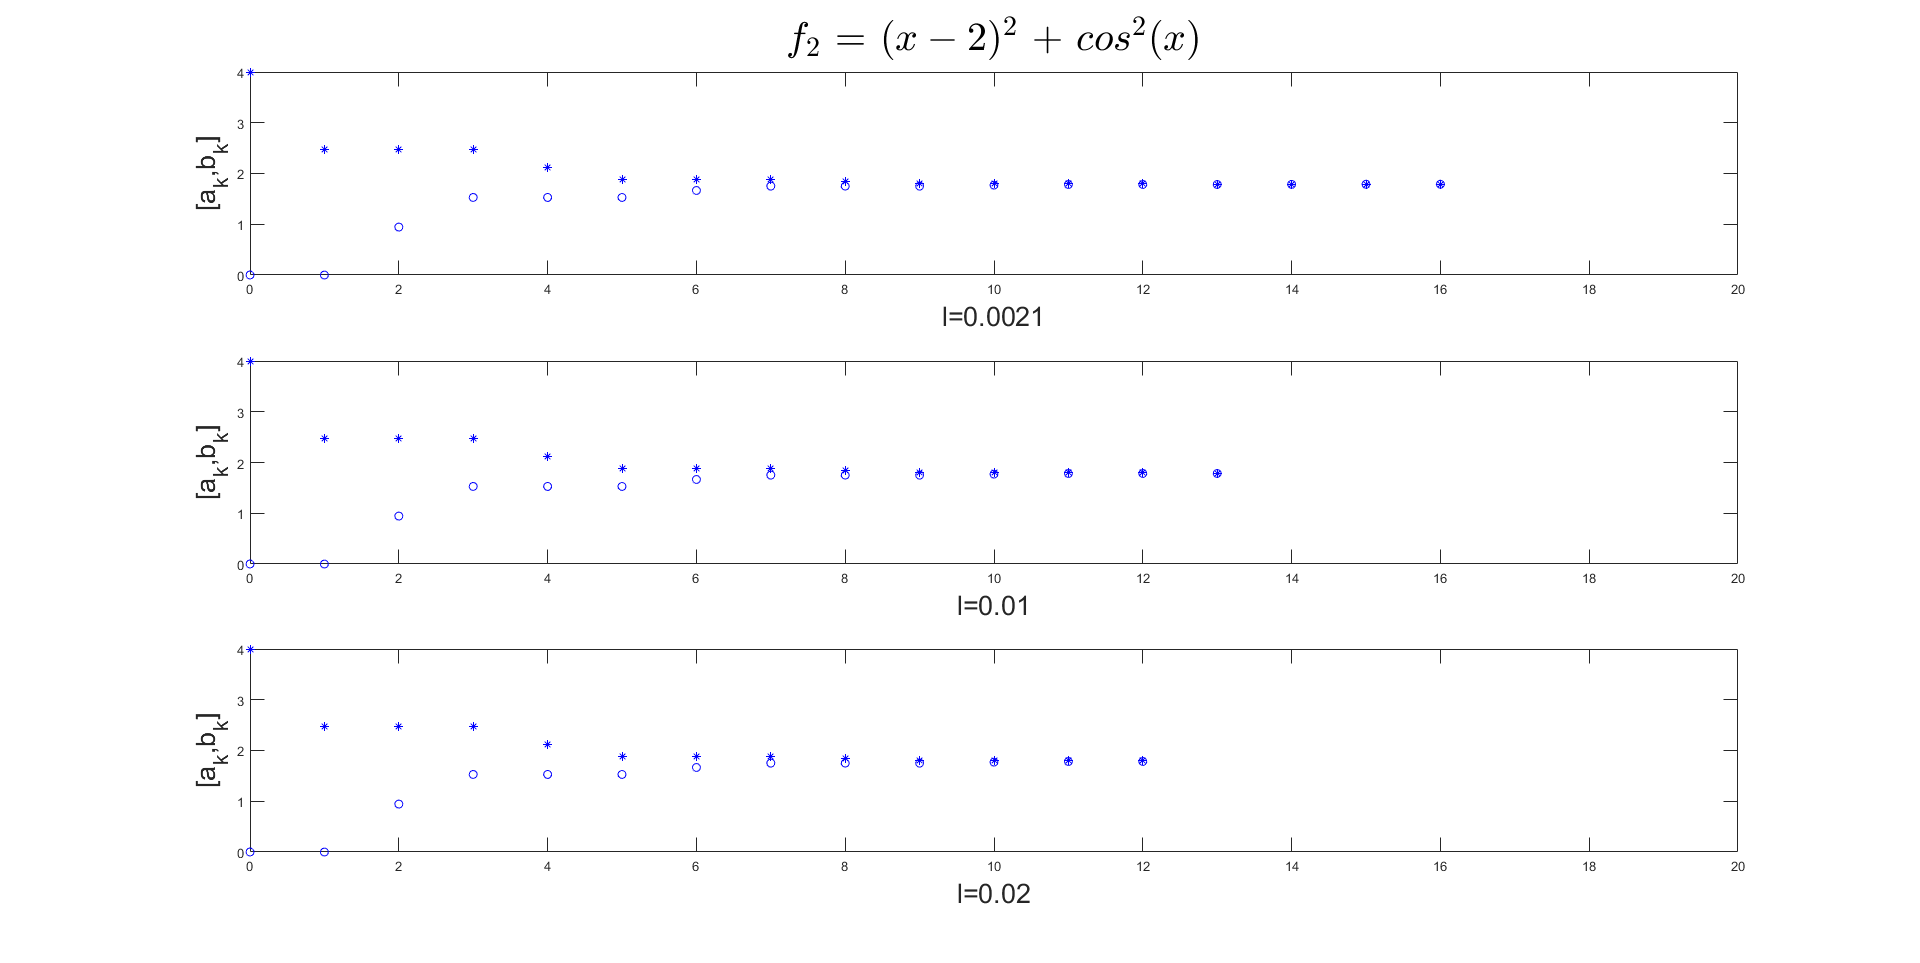
\includegraphics[width=160mm,scale=2]{u2b.png}
\end{figure*} \clearpage
\begin{figure*}[h!]	
     \centering
     \advance\leftskip-2.45cm 
  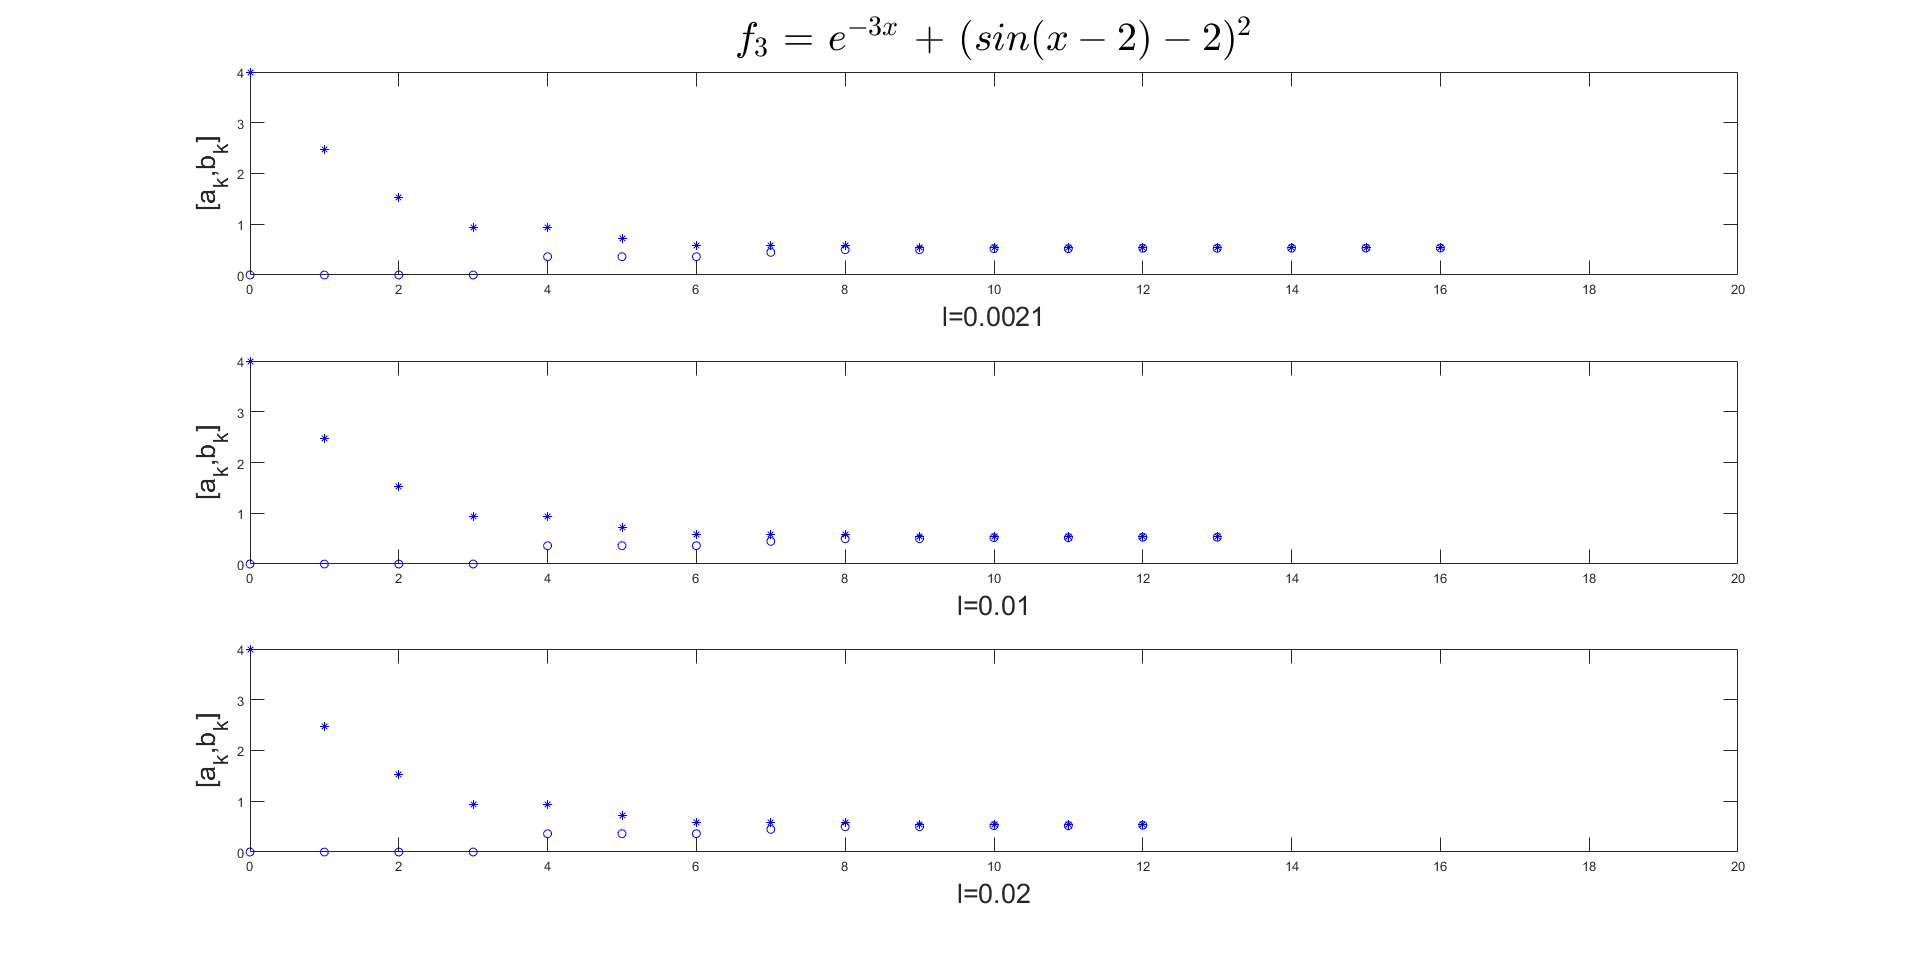
\includegraphics[width=170mm,scale=2]{u2c.png}
\end{figure*}
 όπως φαίνεται απο τα διαγράμματα ο αλγόριθμος συγκλίνει στο ελάχιστο πιο γρήγορα οσο το $l$ μεγαλώνει ωστόσο με μικρότερη ακρίβεια αφού το εύρος που υπάρχει το ελάχιστο μεγαλώνει 
 \newpage
 \section*{Θέμα 3}
 \subsection*{Λίγα λόγια για τον αλγόριθμο} 
Σε αυτό το θέμα θα υλοποιήσουμε στο matlab τη μέθοδο του fibonacci την οποία θα εφαρμόσουμε στις συναρτήσεις και θα σχολιάσουμε τα αποτελέσματα.
 Η μέθοδος fibonacci μοιάζει αρκετά με τη μέθοδο του χρυσού τομέα, βέβαια στη μέθοδο
fibonacci το νέο διάστημα δεν μειώνεται σε σχέση με το προηγούμενο διάστημα με τη βοήθεια
της σταθεράς γ αλλά με τη βοήθεια της ακολουθίας fibonacci. Ο συντελεστής αυτός δεν είναι
σταθερός αλλά αλλάζει σε κάθε επανάληψη. \\
Σε αντίθεση με την σύμβαση του βιβλίου θα πάρουμε την ακουλουθία 
 \[
    F_n = \left\{\begin{array}{lr}
        0, & n=0\\
        1, & n=1\\
        F_{n-1} + F_{n-2}, & n > 1
        \end{array}\right\} 
  \]
\subsection*{Περιγραφή αλγόριθμου}
Δεδομένων των $a_1$ και $b_1$ για k=1 αρχικά υπολογίζουμε την ακολουθία Fibonacci έτσι ώστε $F_n > \frac{b_1 - a_1}{l}$ και στην συνέχεια τα αρχικά σημεία\\ $\boxed{x_{11} = a_1 + \frac{F_{n-k-1}}{F_{n-k+1}}(b_k-a_k)}$ και $\boxed{x_{21} = a_1 + \frac{F_{n-k}}{F_{n-k+1}}(b_k-a_k)}$ \\
Στην συνέχεια σε έναν βρόγχο επανάληψης για n-1 φορές: \\

\begin{equation*}
Αν \enspace f(x1k)< f(x2k) \enspace τoτε \enspace a_{k+1} = a_k \enspace και \enspace b_{k+1} = x_{2k}
\end{equation*}
\begin{equation*}
x_{1k+1} = a_{k+1} + \frac{F_{n-k-2}}{F_{n-k}}(b_{k+1}-a_{k+1}) \enspace και \enspace  x_{2k+1} = x_{1k}
\end{equation*}
 \begin{equation*}
Αν \enspace f(x1k)> f(x2k) \enspace τoτε \enspace a_{k+1} = x_{1k} \enspace και \enspace b_{k+1} = b_{k}
\end{equation*}
\begin{equation*}
x_{2k+1} = a_{k+1} + \frac{F_{n-k-1}}{F_{n-k}}(b_{k+1}-a_{k+1}) \enspace και \enspace  x_{1k+1} = x_{2k}
\end{equation*}
  \subsection*{Υπολογισμοί της αντικειμενικής συνάρτησης}
  Στην πρώτη επανάληψη του αλγορίθμου έχουμε δύο υπολογισμούς της αντικειμενικής συνάρτησης $f(x_{11})$ και $f(x_{21})$ ενώ για κάθε επόμενη επανάληψη έχουμε ένα επιπλέον υπολογισμό. Ωστόσο επειδή ο αλγόριθμος τρέχει για n-1 επαναλήψεις καταλήγουμε οτι oι υπολογισμοί της αντικειμενικής συνάρτησης συνάρτηση του k συνδέονται απο την σχέση:
\begin{equation*}
calc(1) = 2  \enspace για  \enspace k = 1
\end{equation*}
\begin{equation*}
\boxed{calc(k) = k}   \enspace για  \enspace k > 1
\end{equation*}
\newpage
\subsection*{Μεταβολή τελικού ευρους αναζήτησης}
Παρακάτω μελετάμε τη μεταβολή των υπολογισμών της αντικειμενικής συνάρτησης $f_i(x)$
καθώς μεταβάλλουμε το τελικό εύρος αναζήτησης l.
\begin{figure*}[h!]	
     \centering
     \advance\leftskip-4.75cm 
  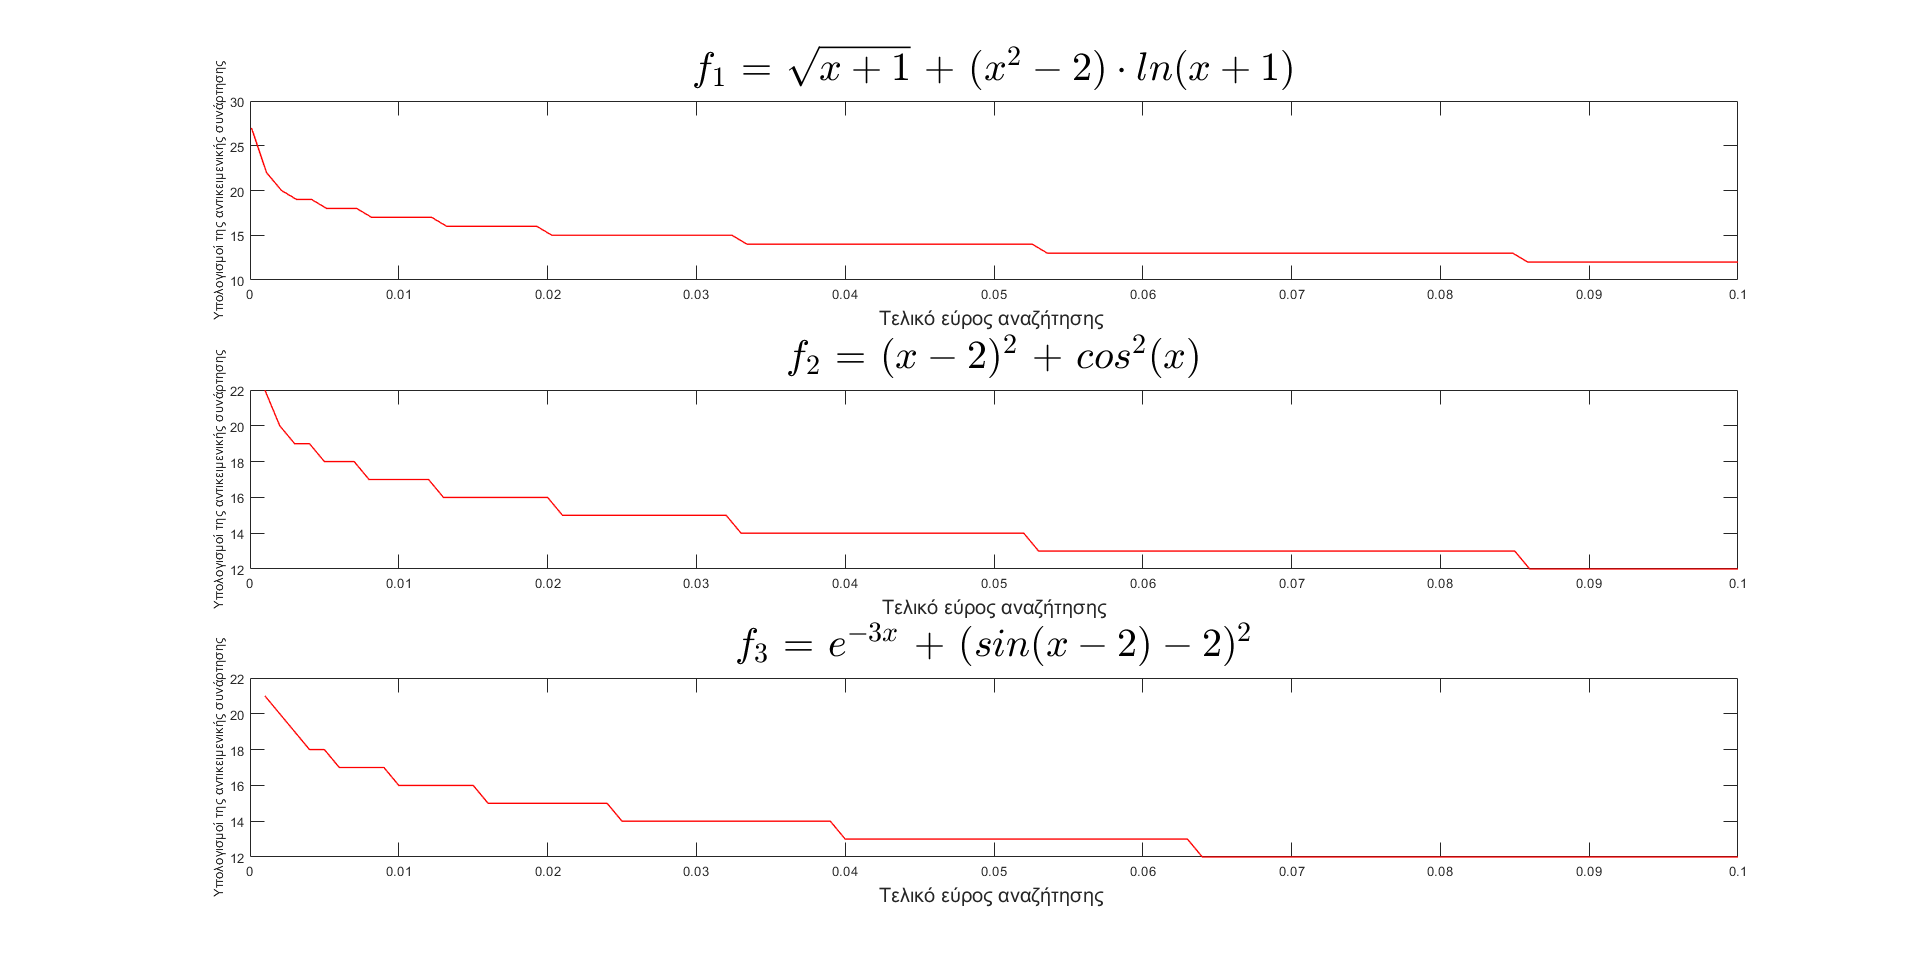
\includegraphics[width=220mm,scale=2]{thema3a.png}
\end{figure*} \\
Βλέπουμε ότι όσο πιο μικρό l δηλαδή όσο μεγαλύτερη ακρίβεια απαιτείται στην εύρεση του
ελαχίστου, τόσο αυξάνονται και οι επαναλήψεις του αλγόριθμου μέχρι τον τερματισμό του, κάτι
απολύτως λογικό.
 \clearpage
  \subsection*{Μεταβολή των υποδιαστημάτων $[a_k,b_k]$}
Tέλος παρουσιάζονται τα διαστήματα $[α_k,b_k]$ ανα επανάληψη $k$ για διάφορα $l$  
\begin{figure*}[h!]	
     \centering
     \advance\leftskip-2.45cm 
  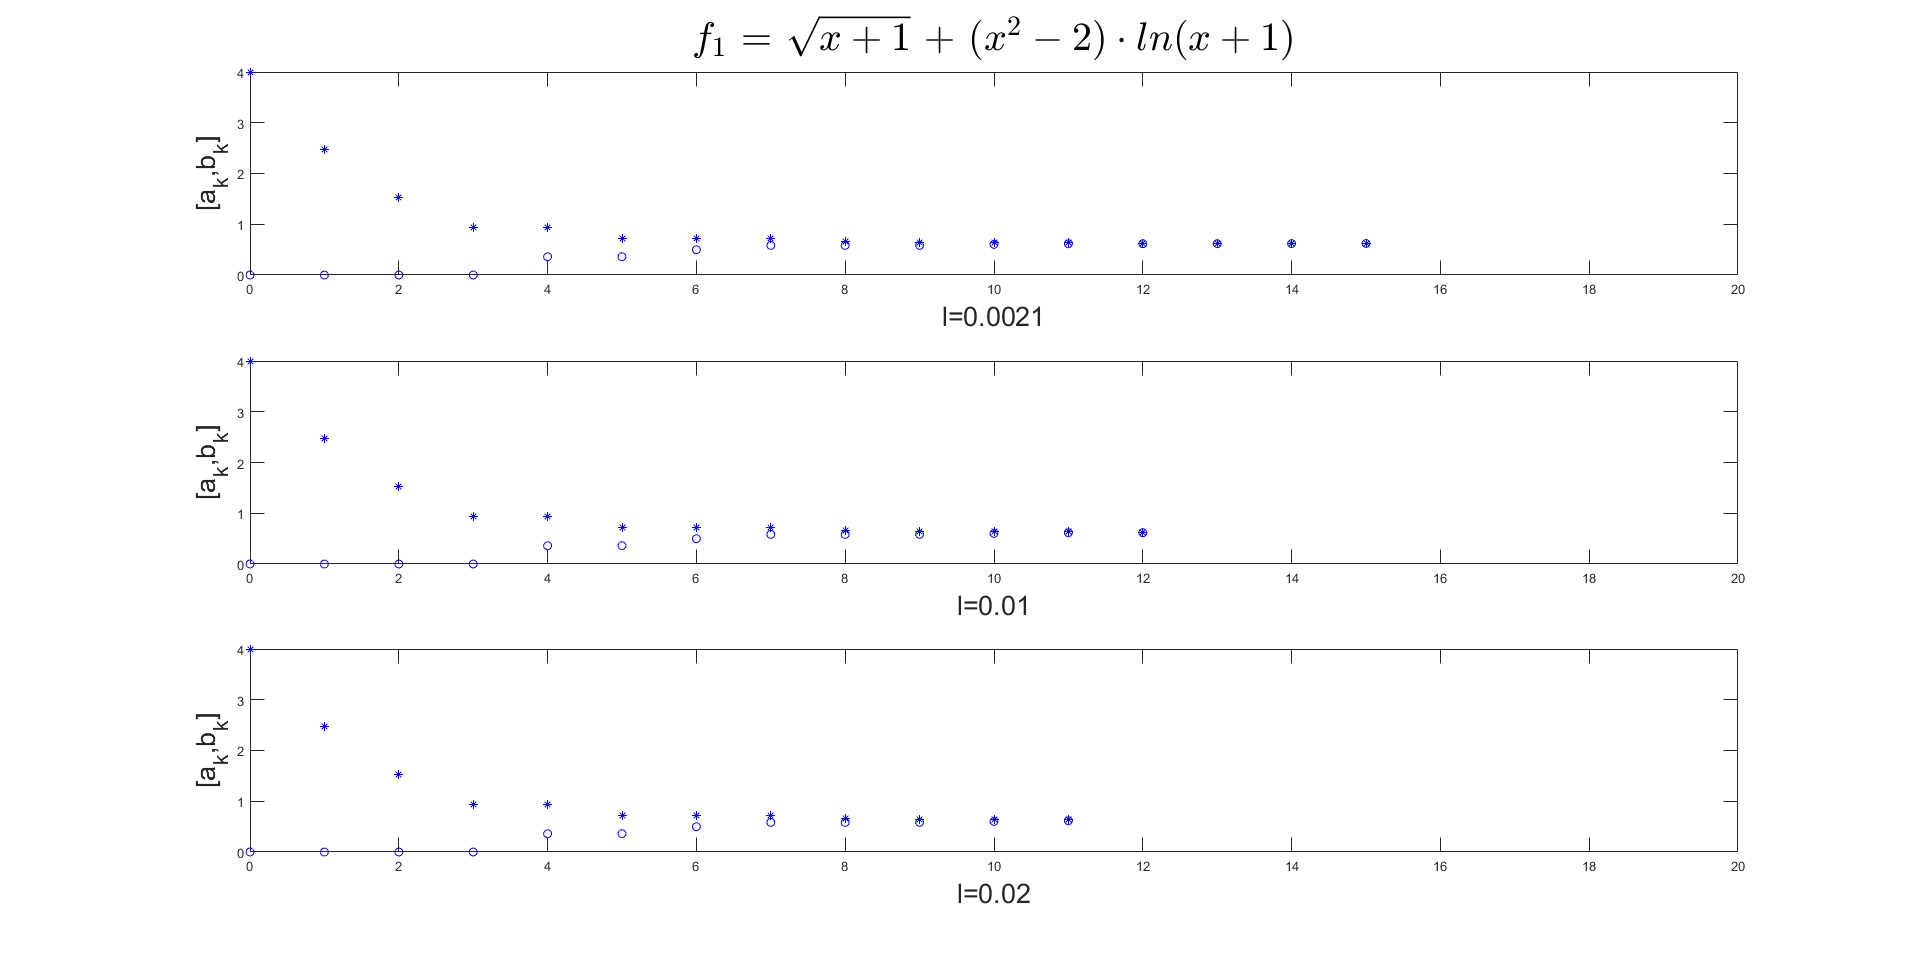
\includegraphics[width=160mm,scale=2]{thema3b1.png}
\end{figure*}
\begin{figure*}[h!]	
     \centering
     \advance\leftskip-2.45cm 
  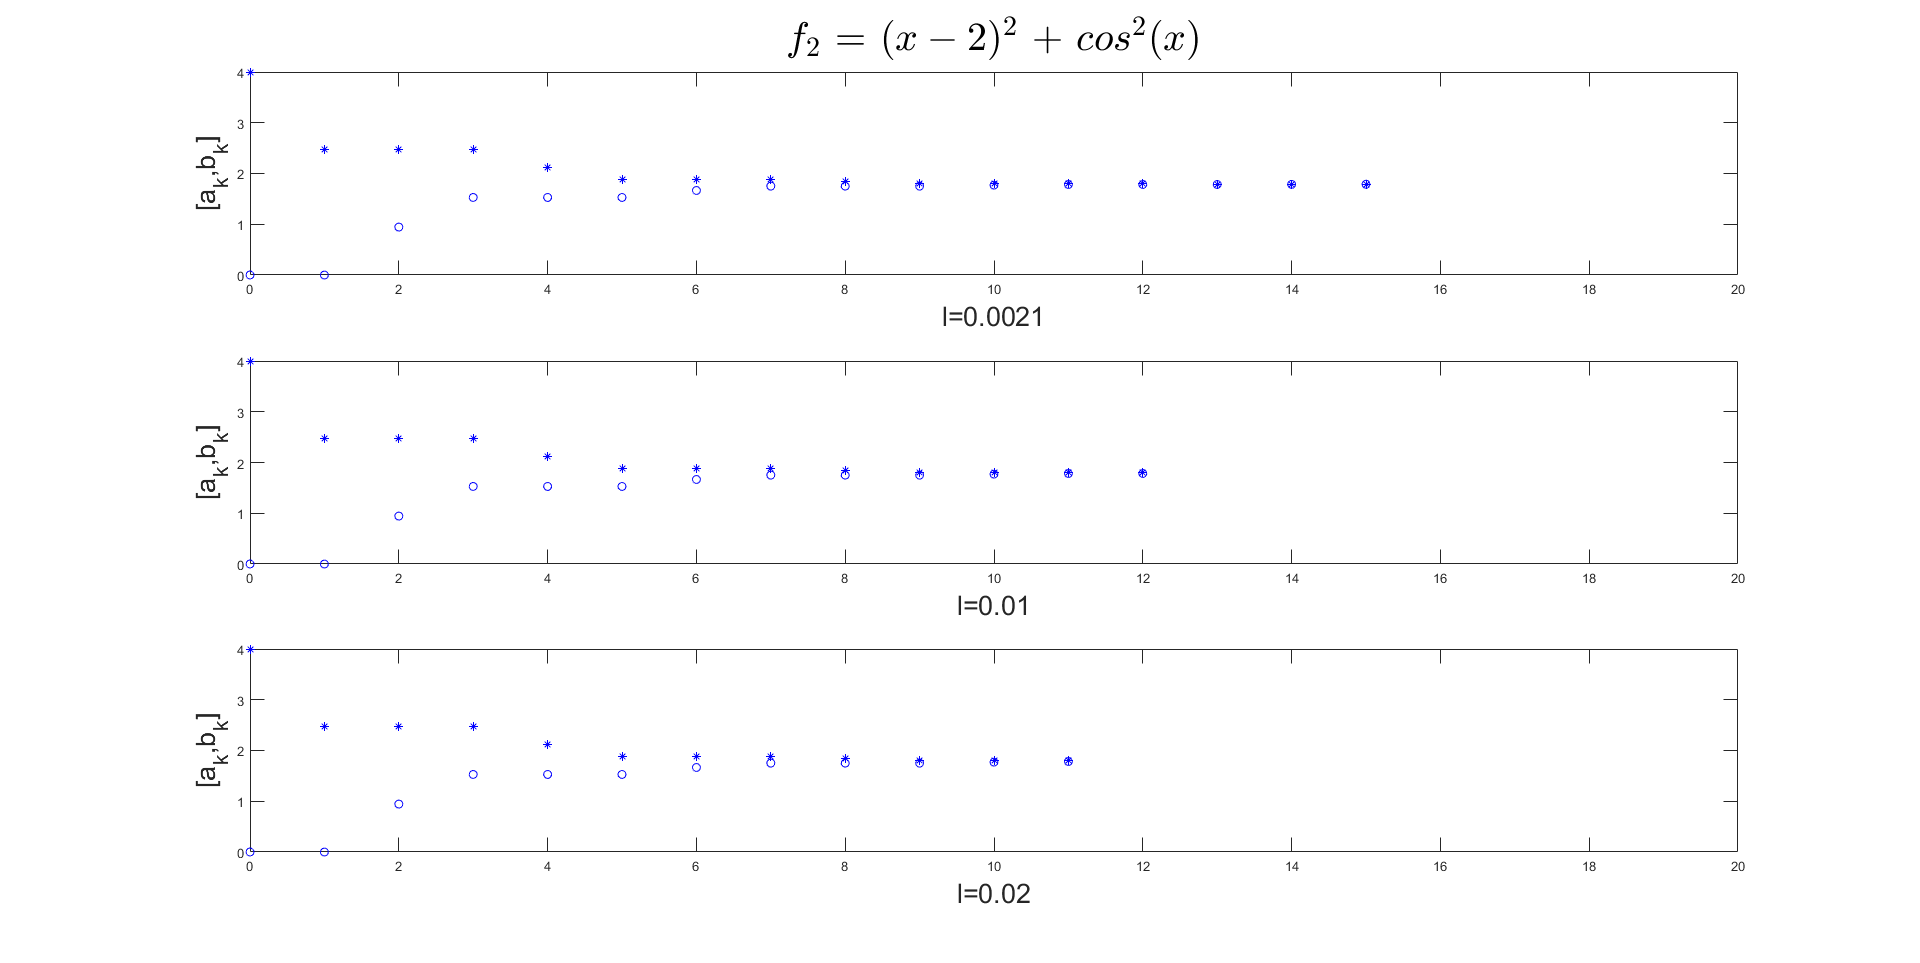
\includegraphics[width=160mm,scale=2]{thema3b2.png}
\end{figure*} \clearpage
\begin{figure*}[h!]	
     \centering
     \advance\leftskip-2.45cm 
  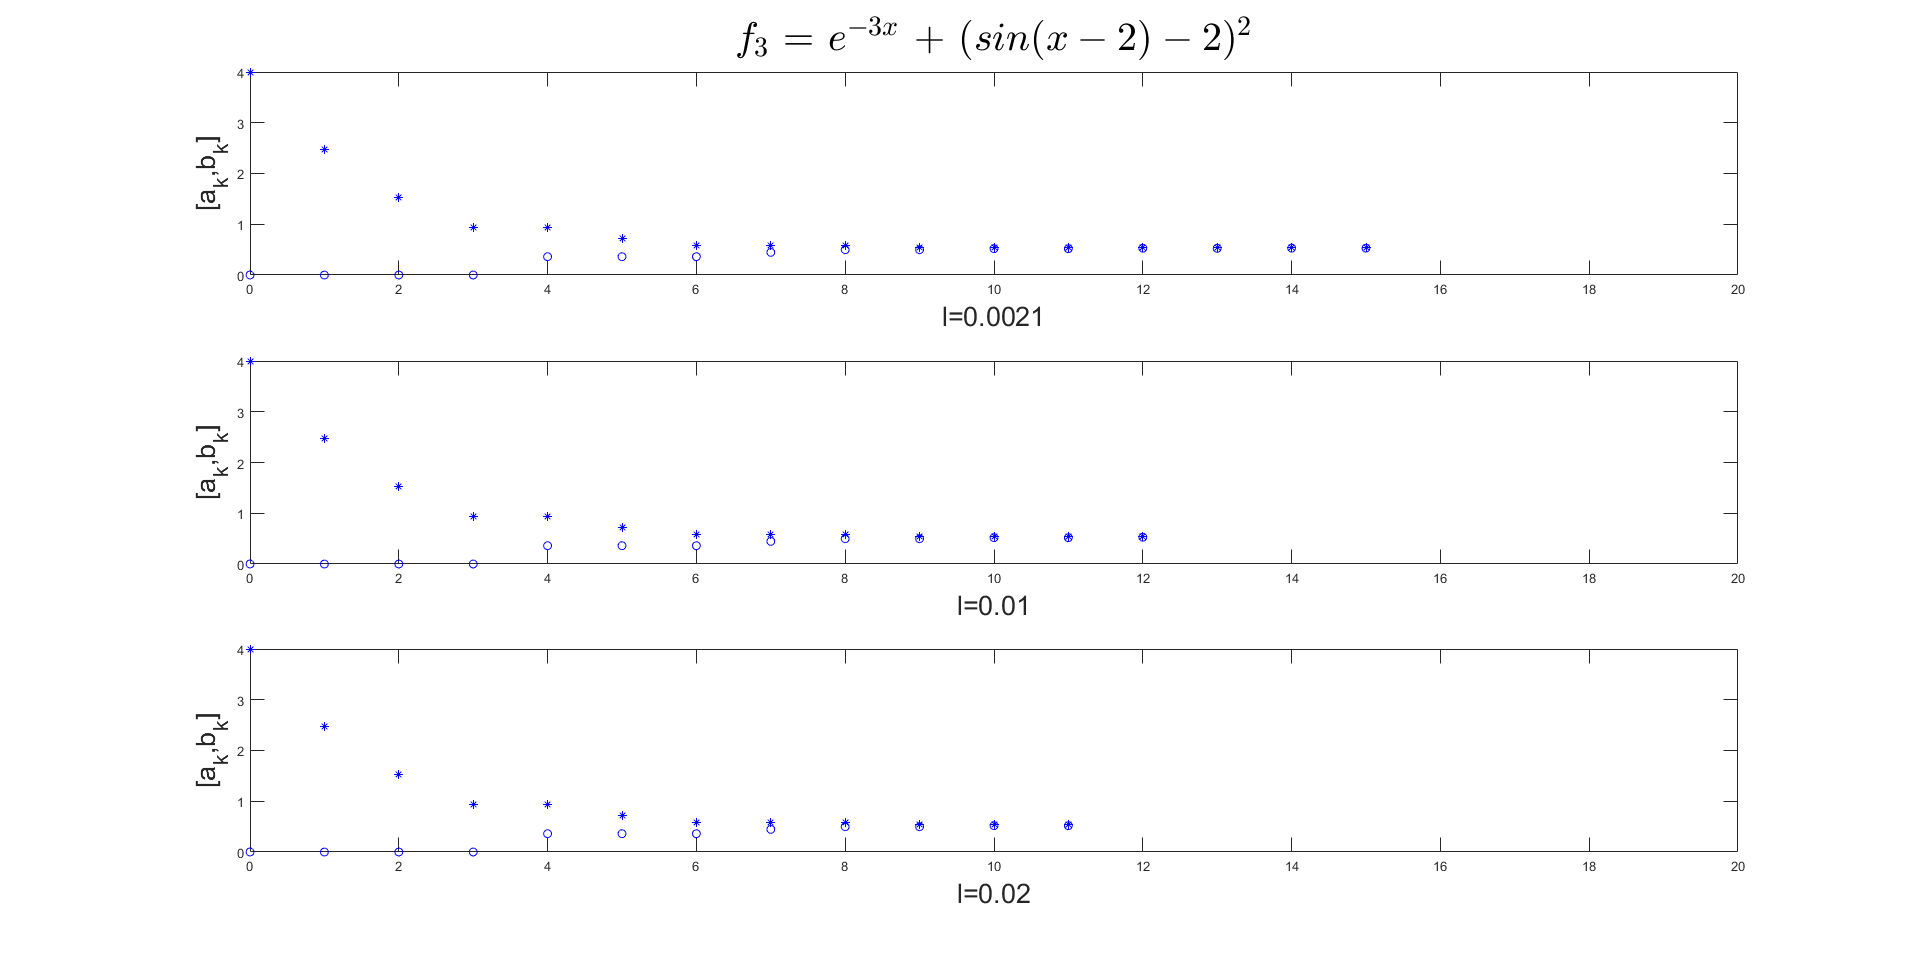
\includegraphics[width=170mm,scale=2]{thema3b3.png}
\end{figure*}
 όπως φαίνεται απο τα διαγράμματα ο αλγόριθμος συγκλίνει στο ελάχιστο πιο γρήγορα οσο το $l$ μεγαλώνει ωστόσο με μικρότερη ακρίβεια αφού το εύρος που υπάρχει το ελάχιστο μεγαλώνει 
 \newpage
  \section*{Θέμα 4}
  \subsection*{Λίγα λόγια για τον αλγόριθμο} 
Σε αυτό το θέμα θα υλοποιήσουμε στο matlab τη μέθοδο του μέθοδο της διχοτόμου με
χρήση παραγώγων την οποία θα εφαρμόσουμε στις συναρτήσεις και θα σχολιάσουμε τα αποτελέσματα.\\
  Επιλέγω $x_k$=($a_k$+$b_k$)/2 , όπου $a_k$, $b_k$ τα άκρα του αρχικού διαστήματος και εξετάζω
το πρόσημο της παραγώγου στο $x_k$. Αν είναι ίση με το μηδέν είμαι στο ελάχιστο, κάτι απολύτως
λογικό γιατί στη μέθοδο θεωρήσαμε κυρτές(σχεδόν) συναρτήσεις. Αν η παράγωγος είναι
μεγαλύτερη του μηδενός τότε το ελάχιστο βρίσκεται αριστερά του $x_k$ και παίρνω σαν νέο
διάστημα [$a_k$,$x_k$] ενώ αν είναι αρνητική το ελάχιστο βρίσκεται δεξιά το $x_k$ και παίρνω σαν νέο
διάστημα το [$x_k$,$b_k$].
\subsection*{Περιγραφή αλγόριθμου}
\begin{equation*}
Aν \enspace \frac{df(x)}{dx} = 0 \enspace για \enspace x = x_k \enspace τοτε \enspace x_k \enspace ειναι \enspace ελαχιστο
\end{equation*}
\begin{equation*}
Αν \enspace \frac{df(x)}{dx} >0 \enspace για \enspace x=x_k \enspace τοτε \enspace [a_{k+1},b_{k+1}] = [a_k,x_k]
\end{equation*}
\begin{equation*}
Αν \enspace \frac{df(x)}{dx} <0 \enspace για \enspace x=x_k \enspace τοτε \enspace [a_{k+1},b_{k+1}] = [x_k,b_k]
\end{equation*}
  \subsection*{Υπολογισμοί της αντικειμενικής συνάρτησης}
Για k=1 έχουμε τον υπολογισμό $\frac{df(x_1)}{dx} \enspace για \enspace x = x_1$ και ο αλγοριθμός ξεκινάει με έναν υπολογισμό αντικειμενικής συνάρτησης. Για κάθε επόμενη επανάληψη προστίθεται πάλι αλλος ένας υπολογισμός αντικειμενικής συνάρτησης συνεπώς καταλήγουμε οτι oι υπολογισμοί της αντικειμενικής συνάρτησης συνάρτηση του k συνδέονται απο την σχέση:
\begin{equation*}
\boxed{calc(k) = k} 
\end{equation*}
Να σημειωθεί πως ο αλγόριθμος έχει τον περιορισμό των επαναλήψεων
\begin{equation*}
(\frac{1}{2})^n \leq \frac{l}{b_1 - a_1}
\end{equation*}
συνεπώς ο αλγόριθμος τερματίζει εως k = n υπολογισμούς 


\newpage

\subsection*{Μεταβολή τελικού ευρους αναζήτησης}
Παρακάτω μελετάμε τη μεταβολή των υπολογισμών της αντικειμενικής συνάρτησης $f_i(x)$
καθώς μεταβάλλουμε το τελικό εύρος αναζήτησης l.
\begin{figure*}[h!]	
     \centering
     \advance\leftskip-4.75cm 
  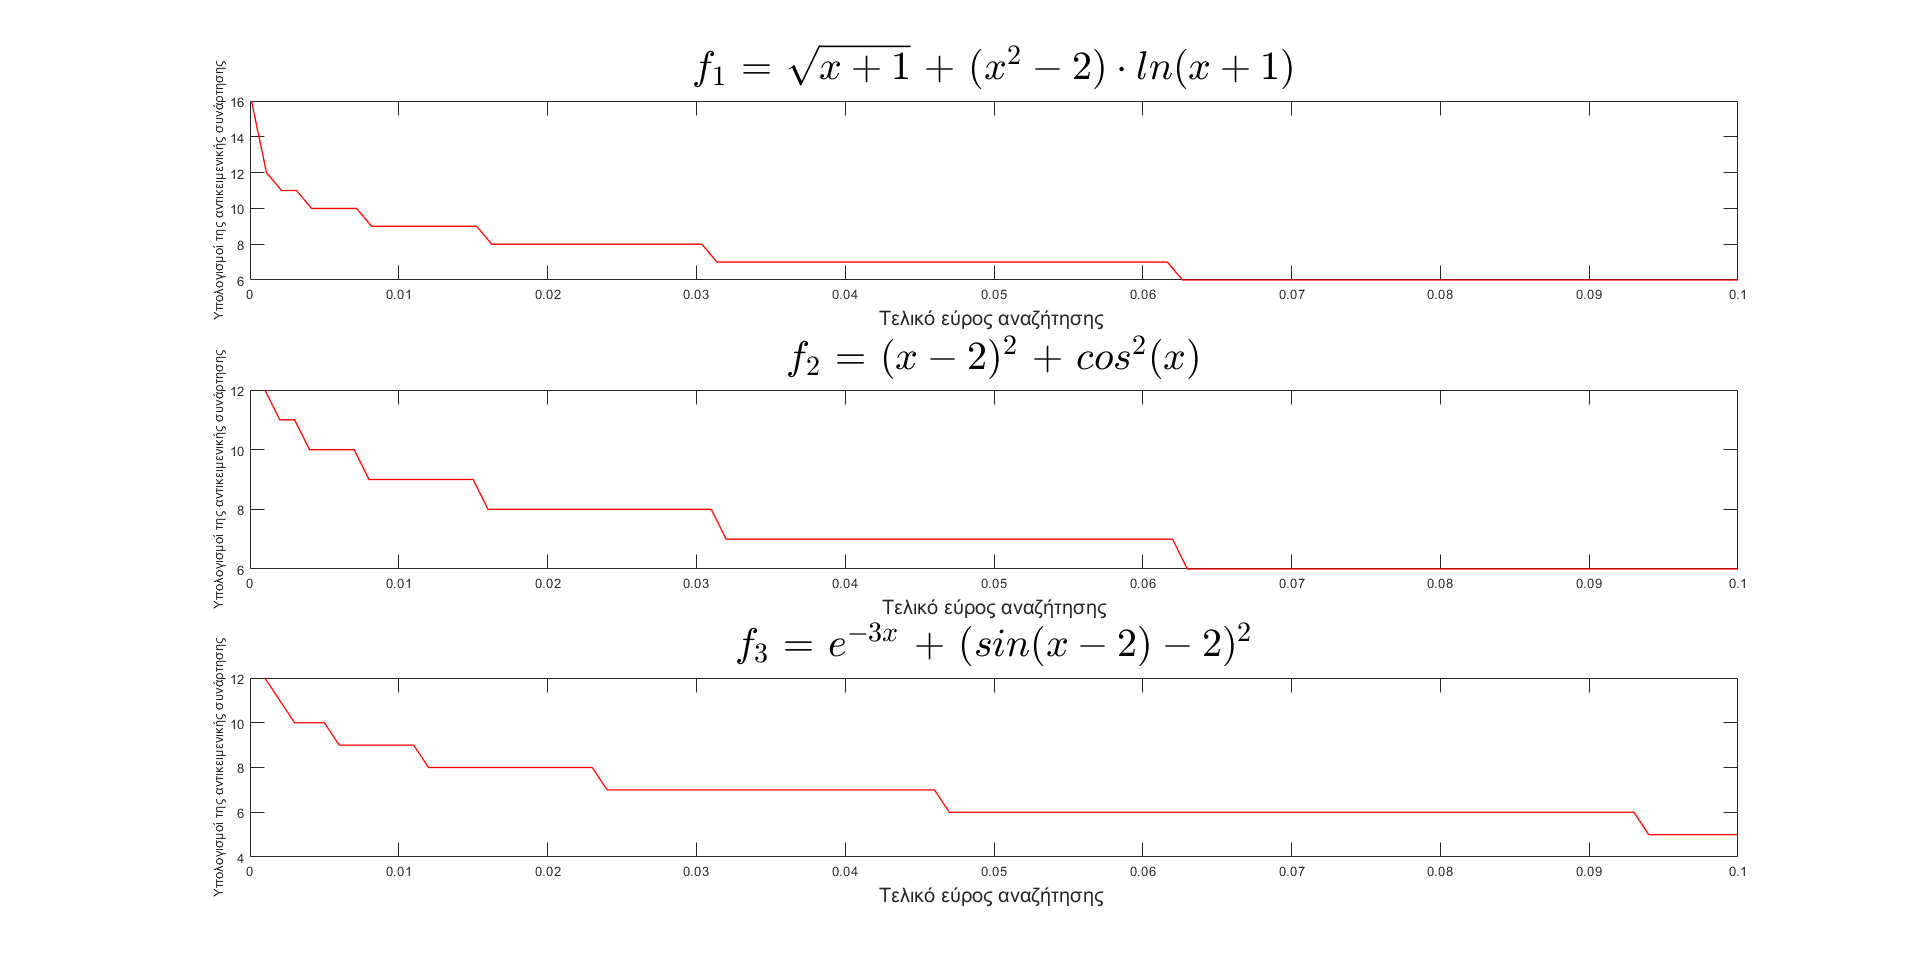
\includegraphics[width=220mm,scale=2]{thema4a.png}
\end{figure*} \\
Βλέπουμε ότι όσο πιο μικρό l δηλαδή όσο μεγαλύτερη ακρίβεια απαιτείται στην εύρεση του
ελαχίστου, τόσο αυξάνονται και οι επαναλήψεις του αλγόριθμου μέχρι τον τερματισμό του, κάτι
απολύτως λογικό.
 \clearpage
  \subsection*{Μεταβολή των υποδιαστημάτων $[a_k,b_k]$}
Tέλος παρουσιάζονται τα διαστήματα $[α_k,b_k]$ ανα επανάληψη $k$ για διάφορα $l$  
\begin{figure*}[h!]	
     \centering
     \advance\leftskip-2.45cm 
  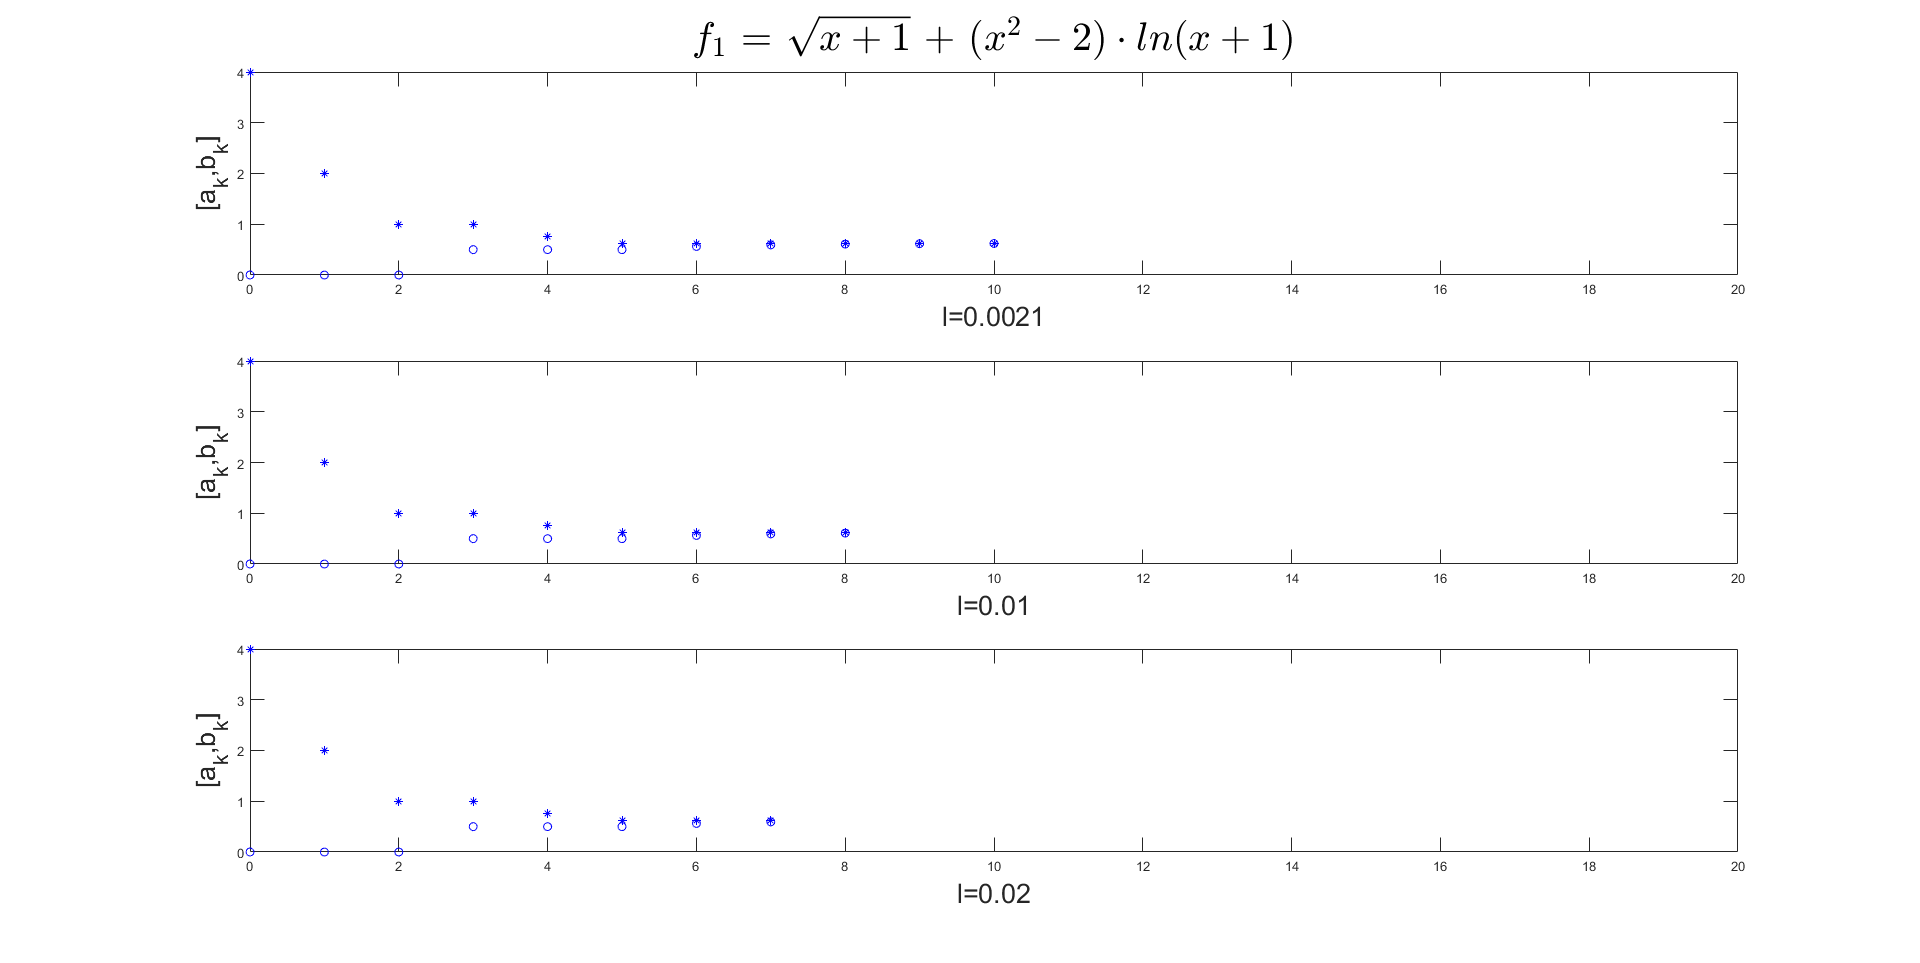
\includegraphics[width=160mm,scale=2]{thema4b1.png}
\end{figure*}
\begin{figure*}[h!]	
     \centering
     \advance\leftskip-2.45cm 
  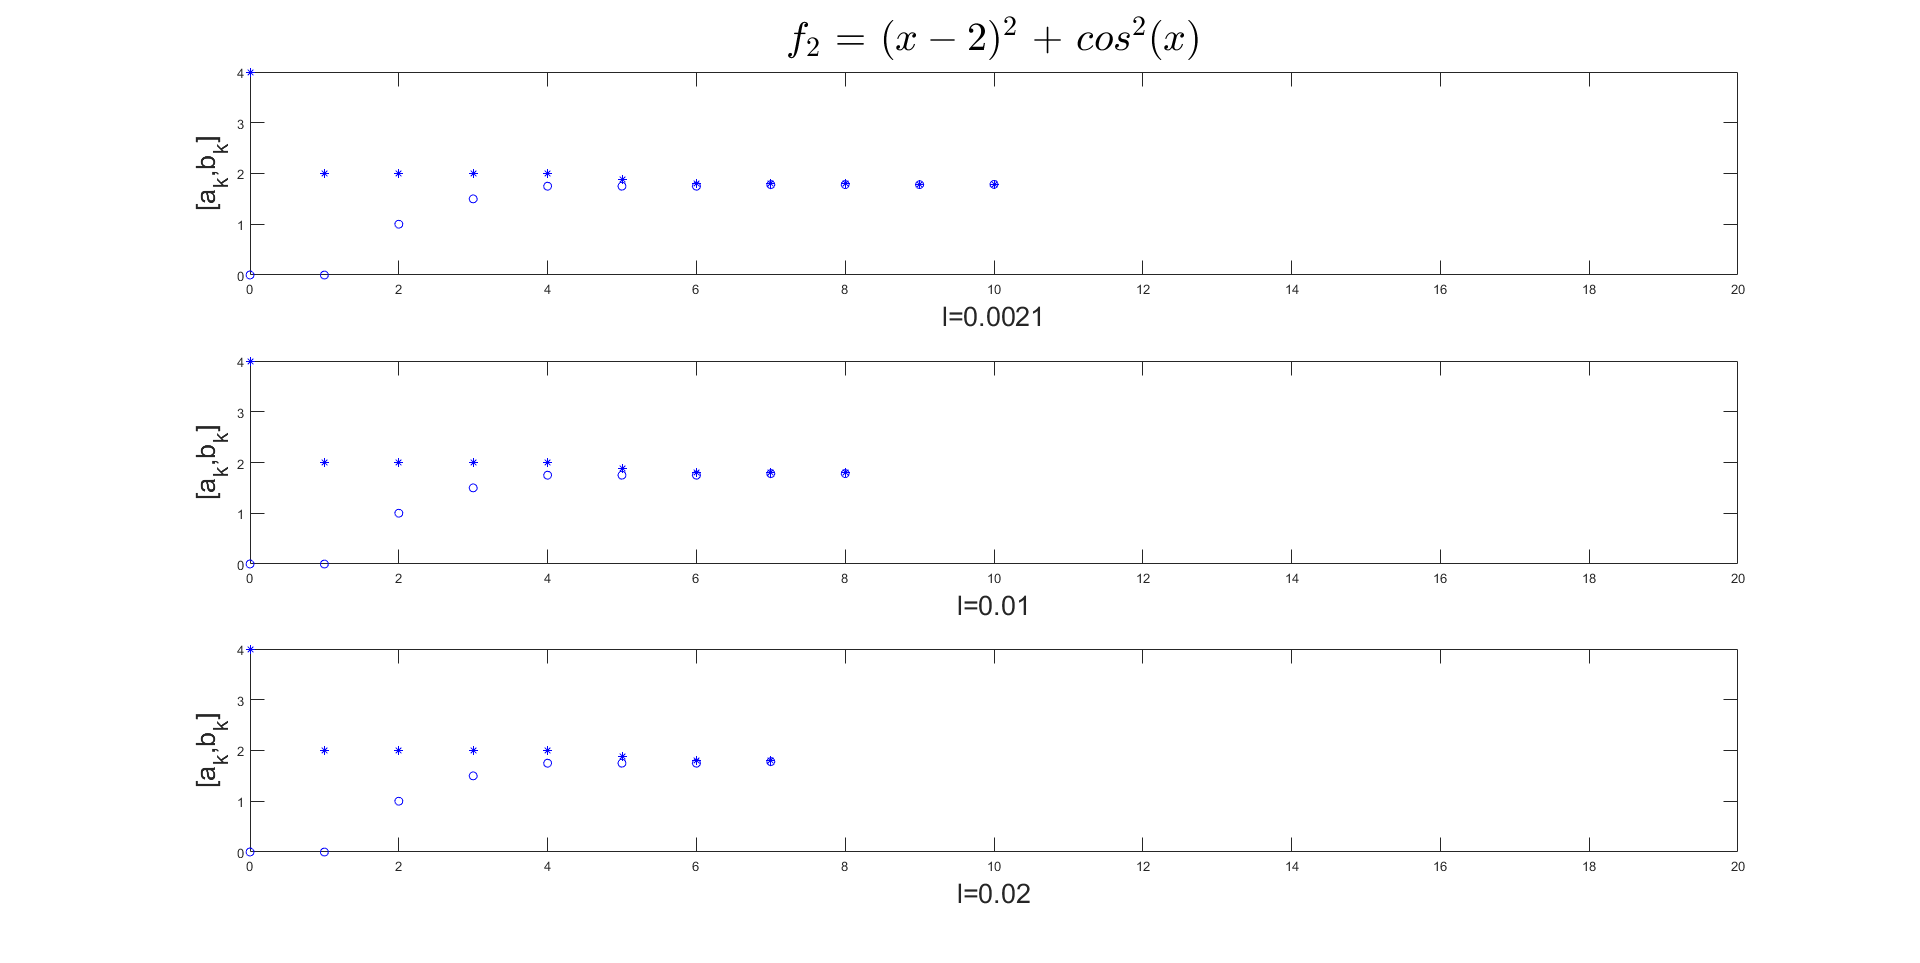
\includegraphics[width=160mm,scale=2]{thema4b2.png}
\end{figure*} \clearpage
\begin{figure*}[h!]	
     \centering
     \advance\leftskip-2.45cm 
  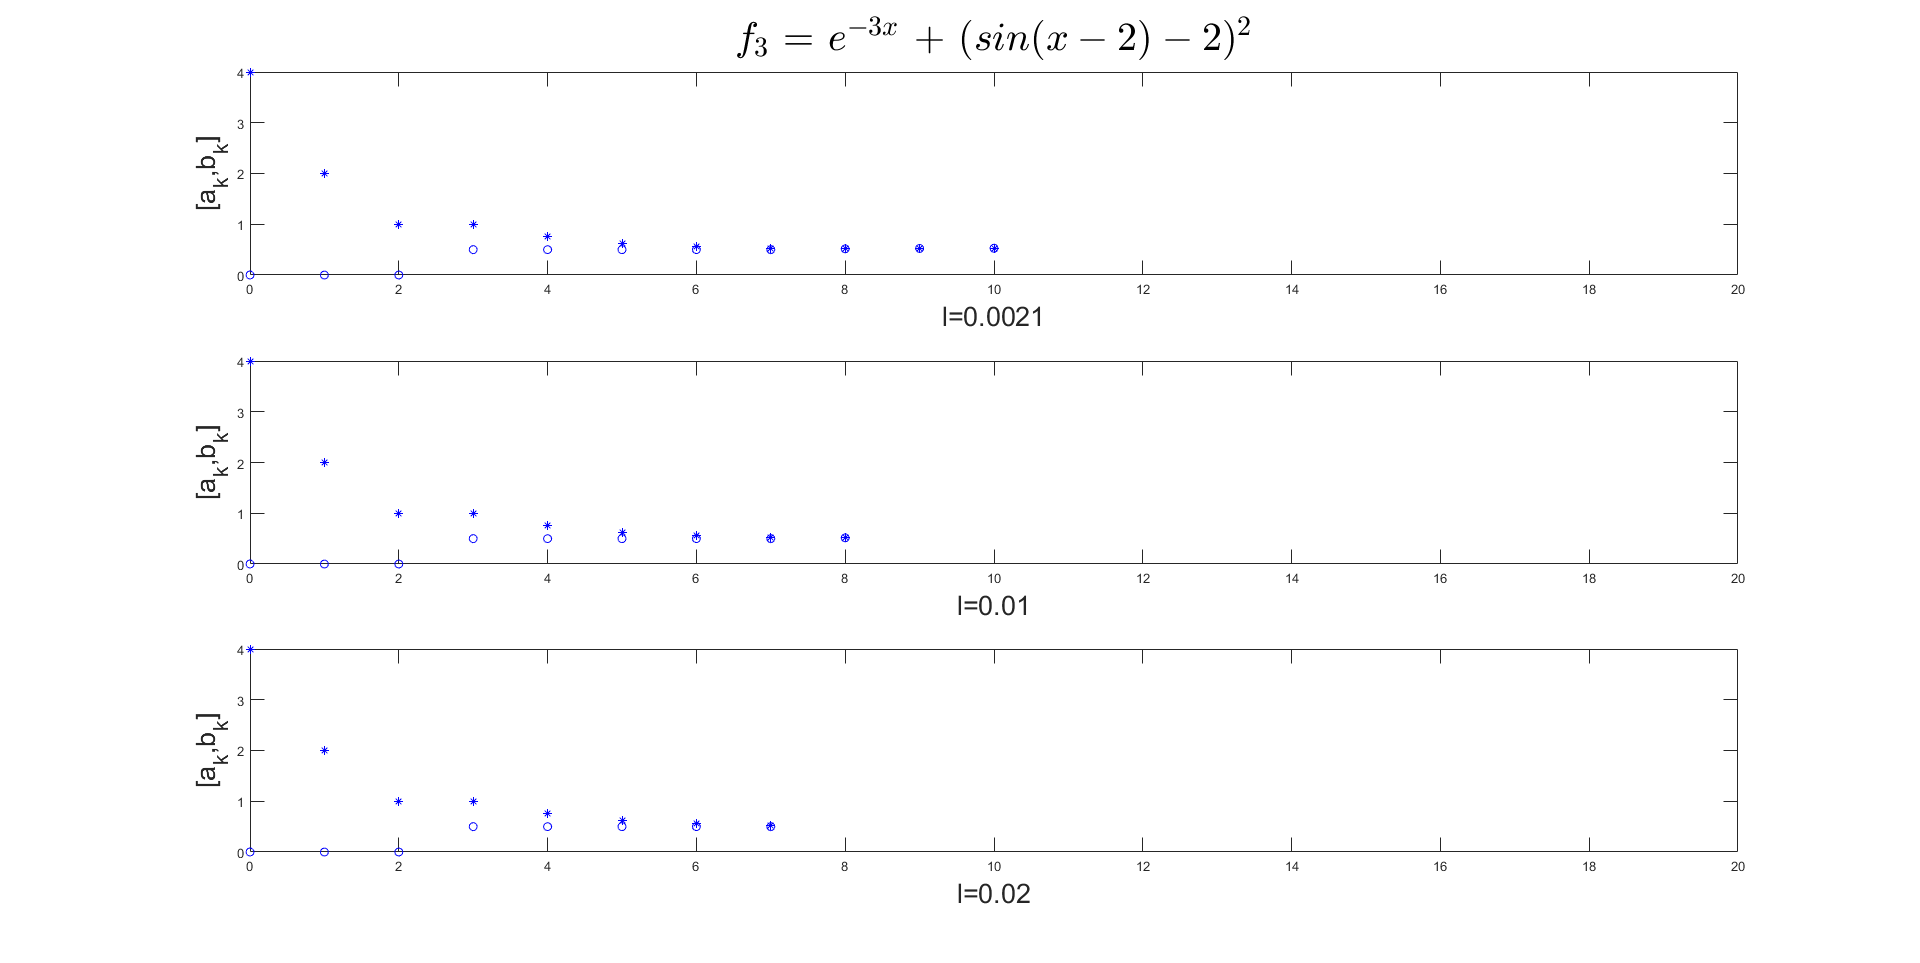
\includegraphics[width=170mm,scale=2]{thema4b3.png}
\end{figure*}
 όπως φαίνεται απο τα διαγράμματα ο αλγόριθμος συγκλίνει στο ελάχιστο πιο γρήγορα οσο το $l$ μεγαλώνει ωστόσο με μικρότερη ακρίβεια αφού το εύρος που υπάρχει το ελάχιστο μεγαλώνει 
 \newpage
 \section*{Σχολιασμός}


\begin{center}
 \begin{tabular}{||c c c c||} 
 \hline
 Algorithm & l=0.0021 & l=0.01 & l=0.02  \\ [0.9ex] 
 \hline\hline
 Διχοτόμησης & 30 & 16 & 14 \\ 
 \hline
 Χρυσής Τομής & 17 & 14 & 13 \\
 \hline
 Fibonacci & 15 & 12 & 11 \\
 \hline
 Παραγώγισης & 10 & 8 & 7 \\
 \hline
 
\end{tabular}
\end{center}
Η
μέθοδος διχοτόμου με χρήση παραγώγων είναι η περισσότερο αποτελεσματική,εν
συνεχεία ακολουθεί η μέθοδος fibonacci, αμέσως μετά η μέθοδος της χρυσής τομής
και τέλος η λιγότερο αποτελεσματική, μέθοδο της διχοτόμου. Τα αποτελέσματα
αυτά συμφωνούν με το βιβλίο Τεχνικές Βελτιστοποίησης.

\end{document}
